\chapter{基于3D点云的缺陷检测}


\section{引言}
金属件的图像采集对打光有严格要求,光源的照射角度以及强度会严重影响检测结果。如一些直射光源会在金属件上产生类似镜面反射的效果,导致采集的二维图像出现“死白”——即一片像素点为无变化特征的白色像素。3D激光相机往往采用蓝光,其能较好降低金属件的反射对成像的影响,有利于特征的提取,为下游缺陷检测提供输入。

在2D缺陷检测领域,PatchCore作为无监督的方法表现出优异的性能。本文基于点云数据的缺陷检测算法受Horwitz等人\cite{horwitzBackFeatureClassical2022}启发,以PatchCore的特征存储为骨干网络,将二维的Patch迁移到三维的Pillar\cite{langPointPillarsFastEncoders2019a},并通过RoPS三维局部特征描述子来提取点云Pillar的特征并进行存储用于检测缺陷。本文称改进的无监督点云缺陷检测方法为PillarCore,算法的整体框架如图\ref{fig:PillarCore}所示。
\begin{figure}[htbp]
    \centering
    \includegraphics[width=1\textwidth]{figures/3/3-framework.pdf}
    \caption{PillarCore框架}\label{fig:PillarCore}
\end{figure}

本章首先将介绍如何组合多种点云滤波方法对输入点云进行预处理,其次将介绍如何通过贪婪投影将点云三角化,接着介绍本文引入的RoPS特征描述子的原理,然后介绍本文基于的PatchCore方法是如何工作的,最后本文展开了多项实验并充分验证说明本文提出的PillarCore算法在无监督点云缺陷检测上的性能表现。



\section{点云预处理}
\subsection{点云直通滤波}

% \begin{figure}[htbp]
%     \centering
%     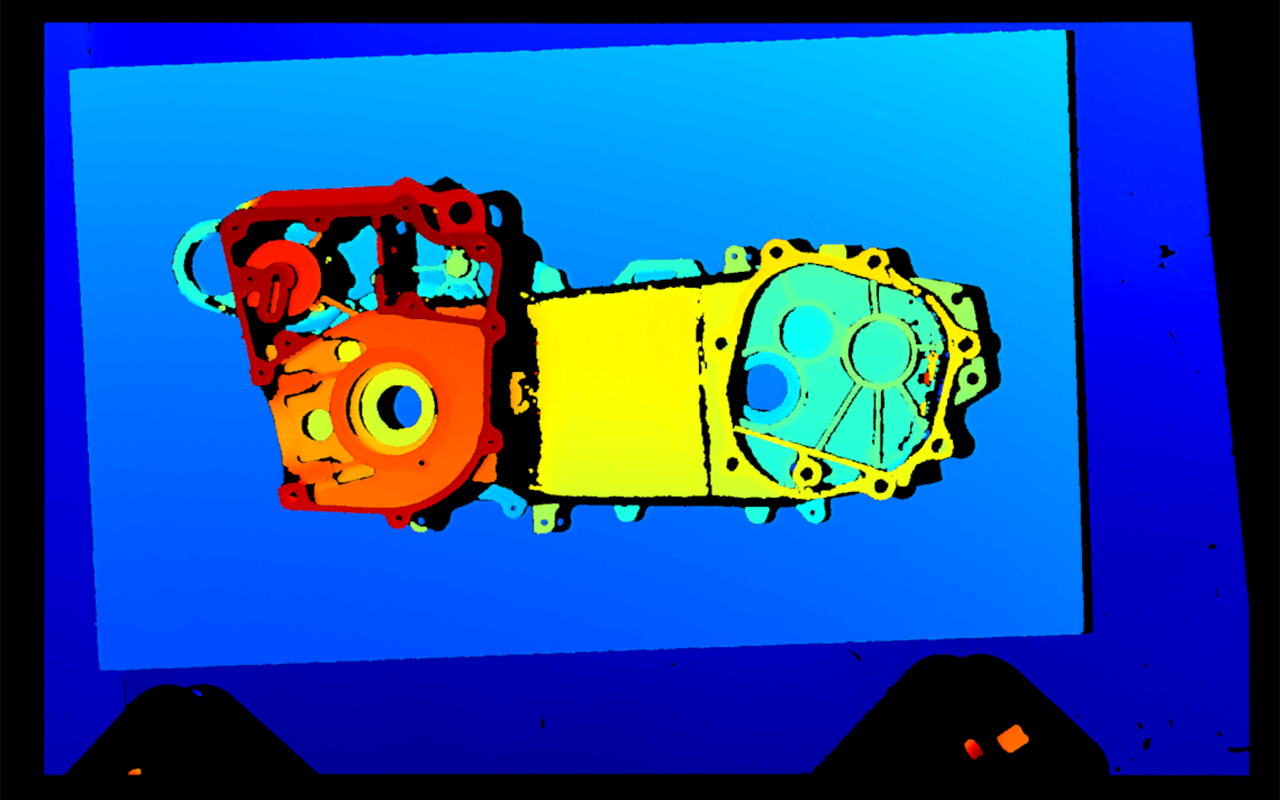
\includegraphics[width=0.75\textwidth]{figures/xy_before_passthrough.png}
%     % \caption[这里的文字将会显示在 listoffigure 中]{这里的文字将会显示在正文中}
%     \caption{原始点云俯视图}\label{fig:xy_before_passthrough}
% \end{figure}

\begin{figure}[htbp]
    \centering
    \begin{subfigure}
        \centering
        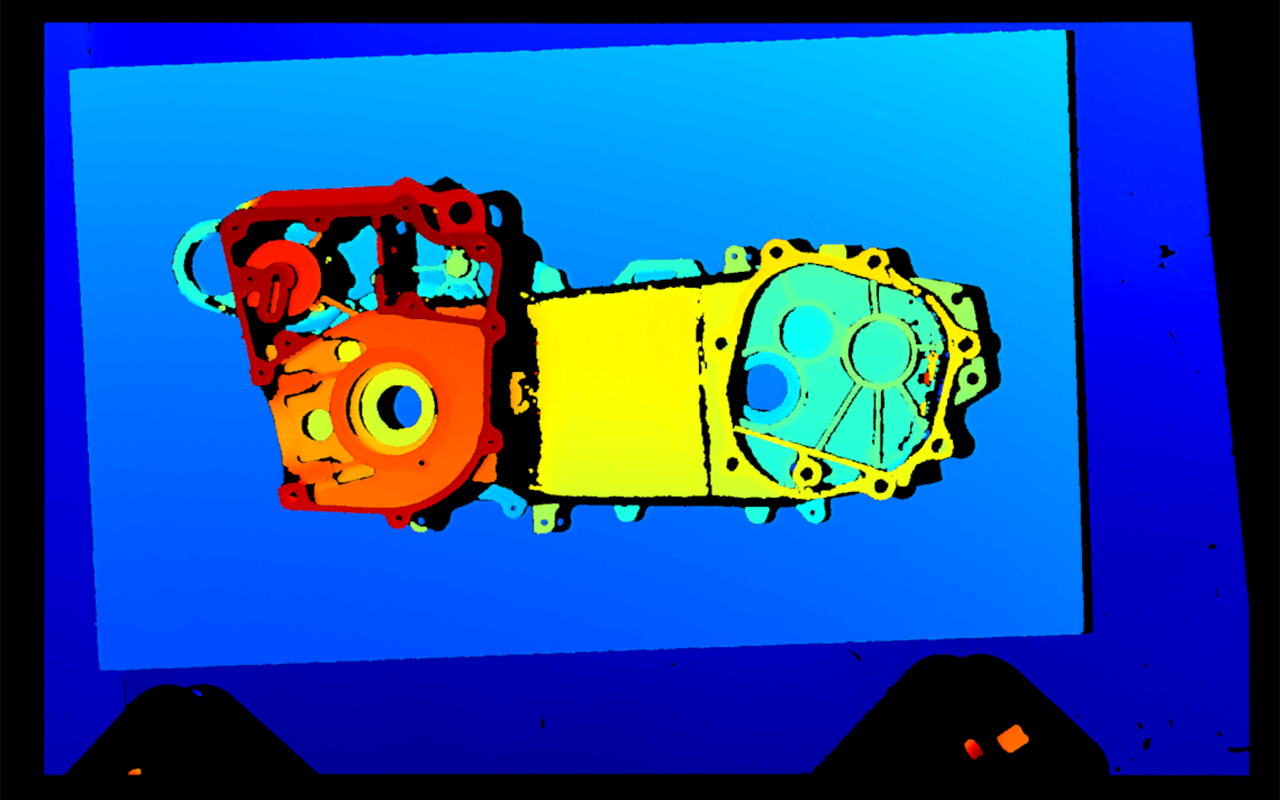
\includegraphics[width=.45\linewidth]{figures/xy_before_passthrough.png}  
      \end{subfigure}
      \begin{subfigure}
        \centering
        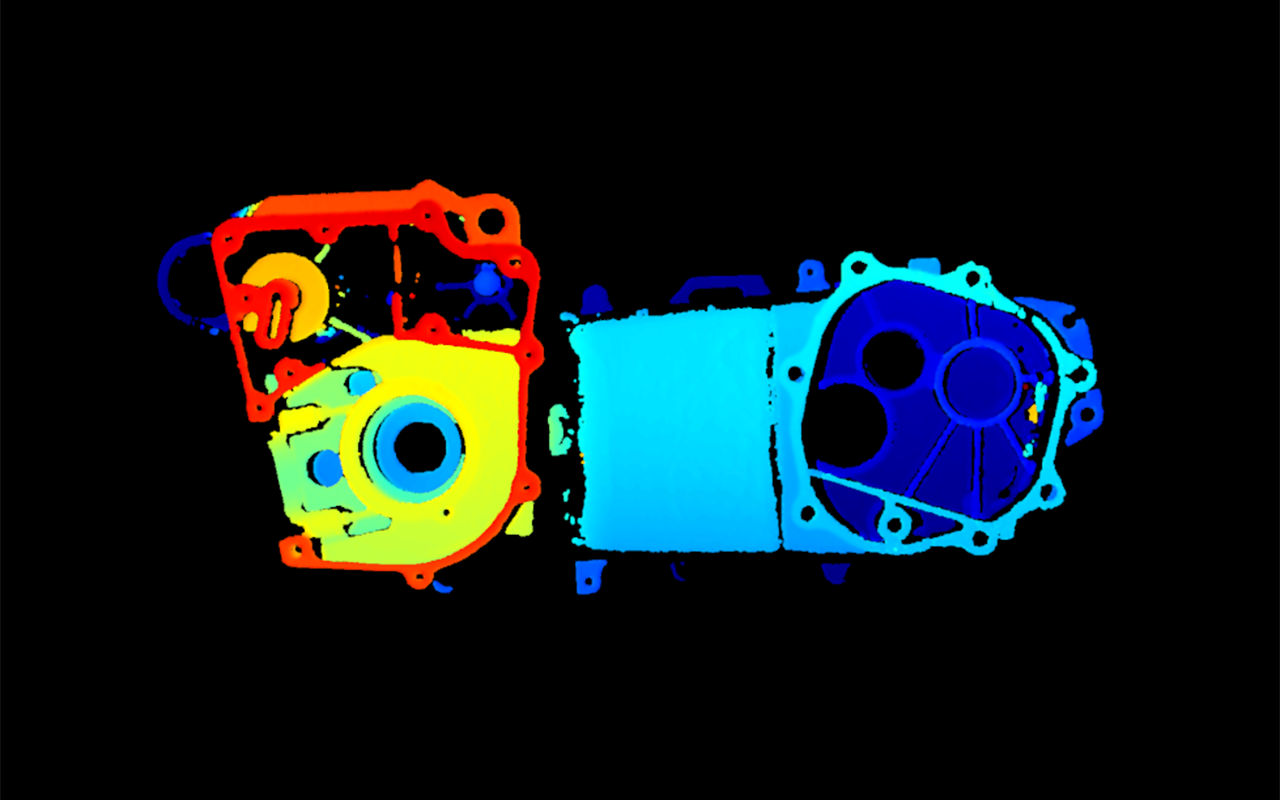
\includegraphics[width=.45\linewidth]{figures/z_xy_afterpassthrough.png} 
      \end{subfigure}
    \caption{直通滤波前后效果}
    \label{fig:xy}
\end{figure}

本文为覆盖多种目标,使用的相机FOV较大,因此会有较多与目标缺陷检测无关的背景被同时采集,如图\ref{fig:xy}中左图所示。直通滤波是一种高效易用的点云滤波方法,其原理是将所有点在指定维度上(如x,y,z轴)与设定的最小值和最大值进行比较,只有在范围内或范围外的点才被保留,其它点则被过滤掉。

直通滤波主要有两大作用。一是通过对点云数据进行直通滤波,能快速去除偏差较大的离群点,降低噪声对后续缺陷检测任务计算结果的影响;二是在点云处理中,直通滤波可以根据设定的范围提取出感兴趣区域的点云,从而实现缩小点云规模,减少后续任务计算量,提高计算效率。
\begin{figure}[htbp]
    \centering
    \begin{subfigure}
        \centering
        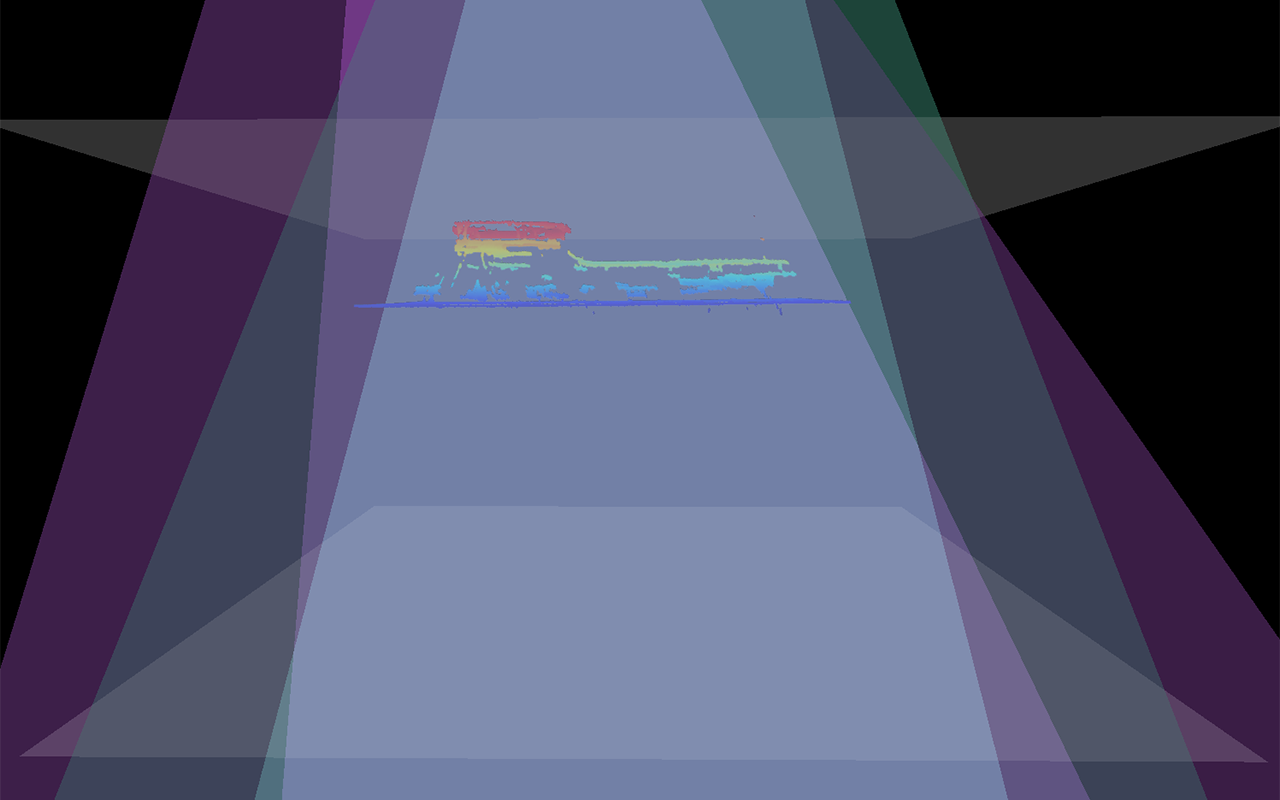
\includegraphics[width=.45\linewidth]{figures/z_before_passthrough.png}  
      \end{subfigure}
      \begin{subfigure}
        \centering
        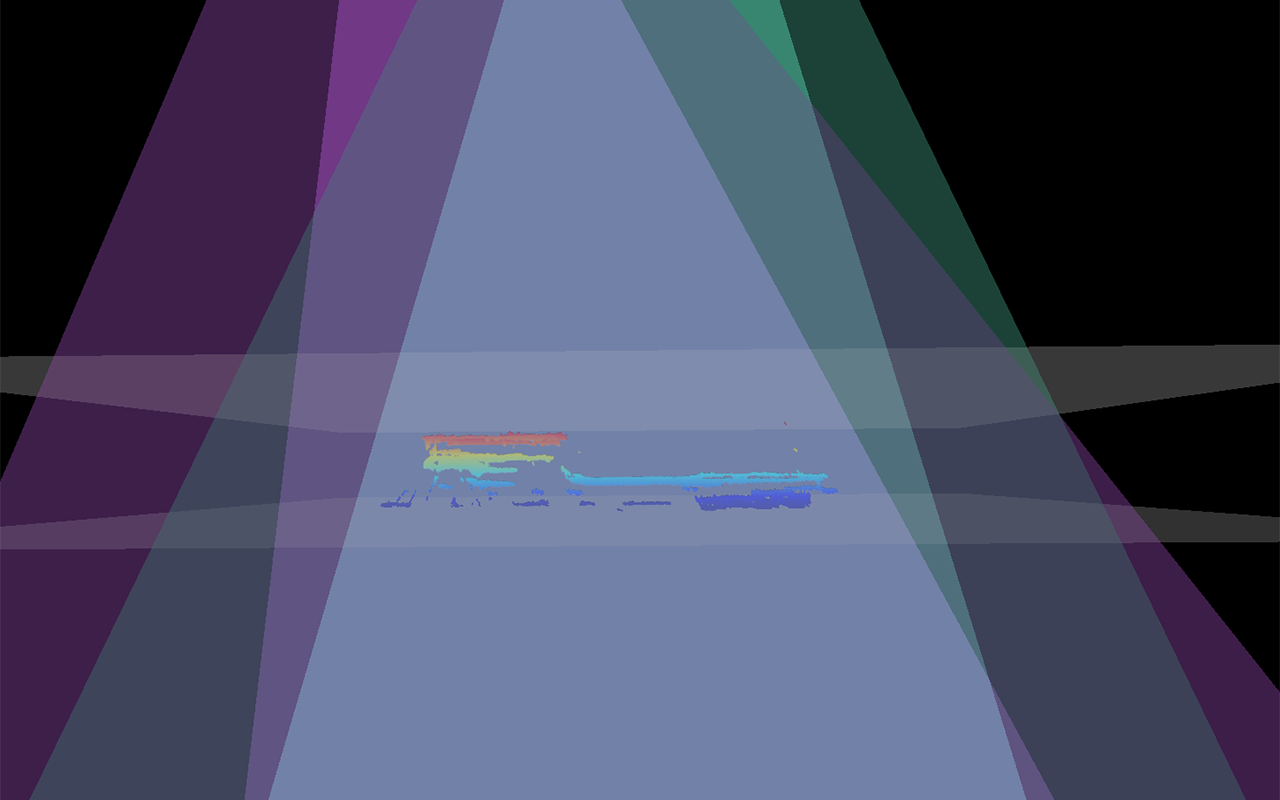
\includegraphics[width=.45\linewidth]{figures/z_after_passthrough.png} 
      \end{subfigure}
    \caption{z轴直通滤波示意图}
    \label{fig:z}
\end{figure}

因此,直通滤波方法常见于各种点云算法的预处理阶段,用来提升算法输入点云的质量。本文研究的对象近似为空间中的立方体,通过分别沿x,y和z轴对点云数据进行直通滤波的预处理,可以实现提取后续缺陷检测任务的ROI区域。其中Z轴直通滤波示意如图\ref{fig:z}所示。

% \begin{figure}[htbp]
%     \centering
%     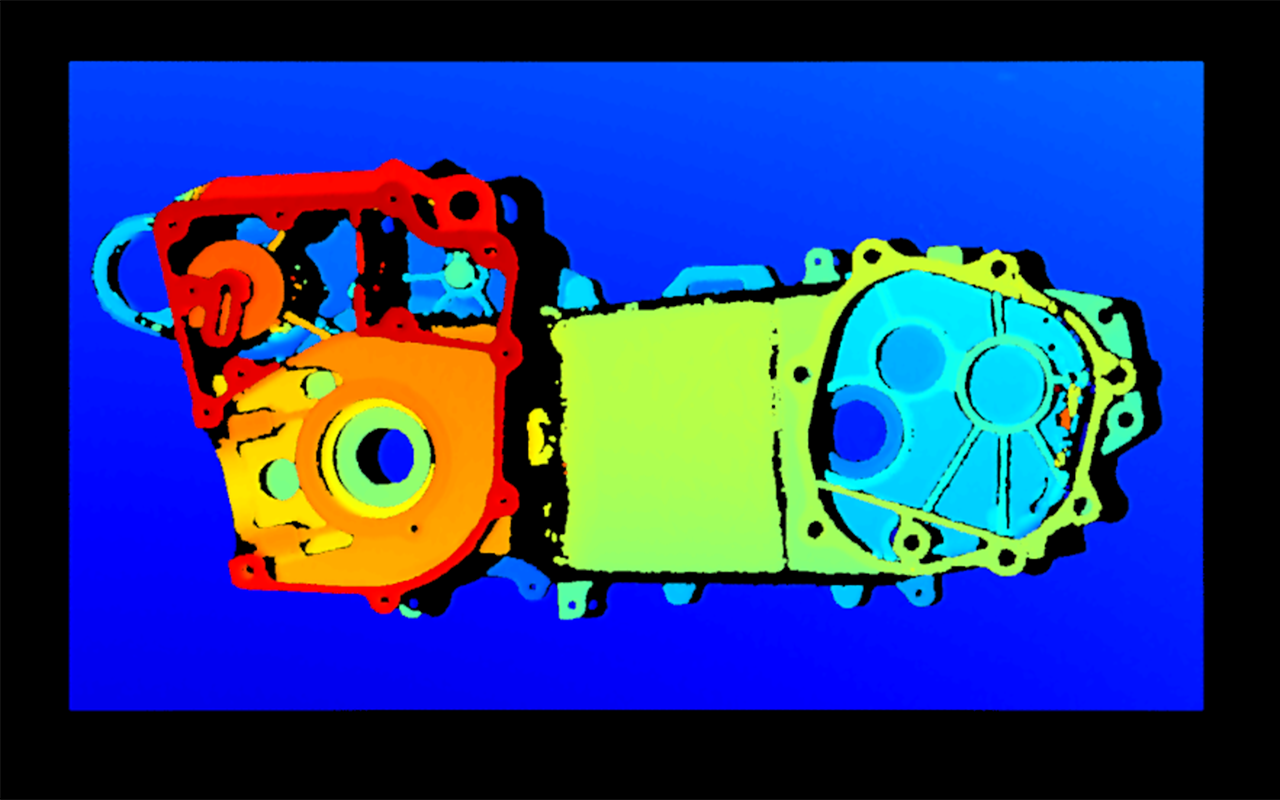
\includegraphics[width=0.75\textwidth]{figures/xy_after_passthrough.png}
%     \caption{按x、y轴对点云直通滤波后俯视图}\label{fig:xy_after_passthrough}
% \end{figure}



% \begin{figure}[htbp]
%     \centering
%     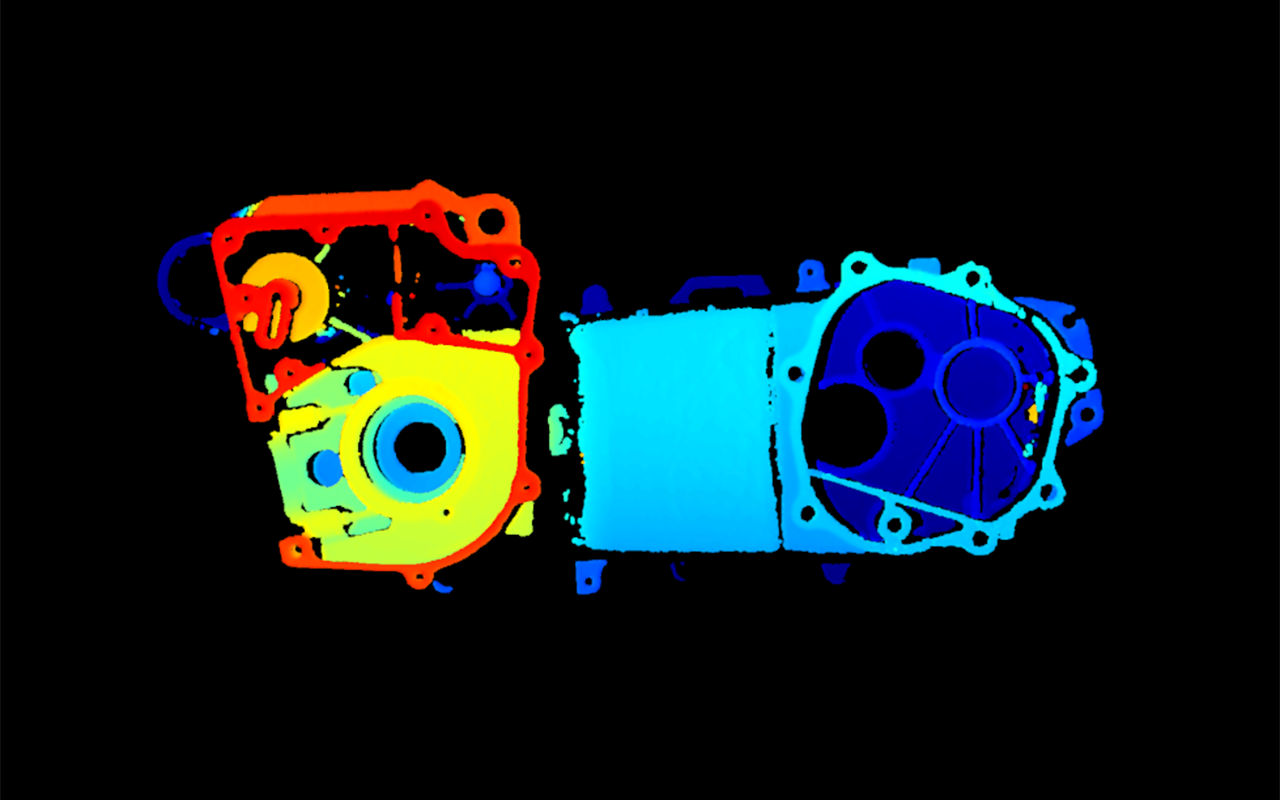
\includegraphics[width=0.75\textwidth]{figures/z_xy_afterpassthrough.png}
%     \caption{按z轴对点云直通滤波后俯视图}\label{fig:z_xy_afterpassthrough}
% \end{figure}



\subsection{点云统计滤波}
离群点是指与其余数据显著不同的点,通常是测量误差或其他异常的结果。本文使用的光栅结构光相机,在采集过程中,面对反光严重的金属件,相机输出的点云数据中存在不少肉眼可观察的离群点,可以预见会对后续缺陷检测任务的准确性和效率产生较大影响。

点云统计滤波是一种用于减少点云数据中噪声的技术,其原理是通过分析数据的统计属性并剔除被判定为离群点的点来实现。点云数据有几种可用的统计滤波器,包括均值、中位数、标准偏差和方差滤波器。这些滤波器都基于数据的统计属性进行操作。

点云统计滤波包括三个主要步骤:数据预处理、统计分析和数据滤波。首先是对点云数据进行预处理,即将原始点云数据转换为可以由统计滤波算法处理的矩阵或数组格式。当数据经过预处理后,接着就可以进行统计分析。常见的统计属性包括均值、中位数、标准偏差和方差等,这些统计属性然后被用来识别离群点。

最后一步是通过删除已识别的离群点来过滤数据。所使用的具体滤波算法将取决于数据的统计属性和应用程序。统计滤波输出的结果是一个已经清理噪声且更适合进一步处理的点云数据集,其效果如图\ref{fig:statistic}所示,其中红色标记的点是统计滤波滤出的离群噪声点。
\begin{figure}[htbp]
    \centering
    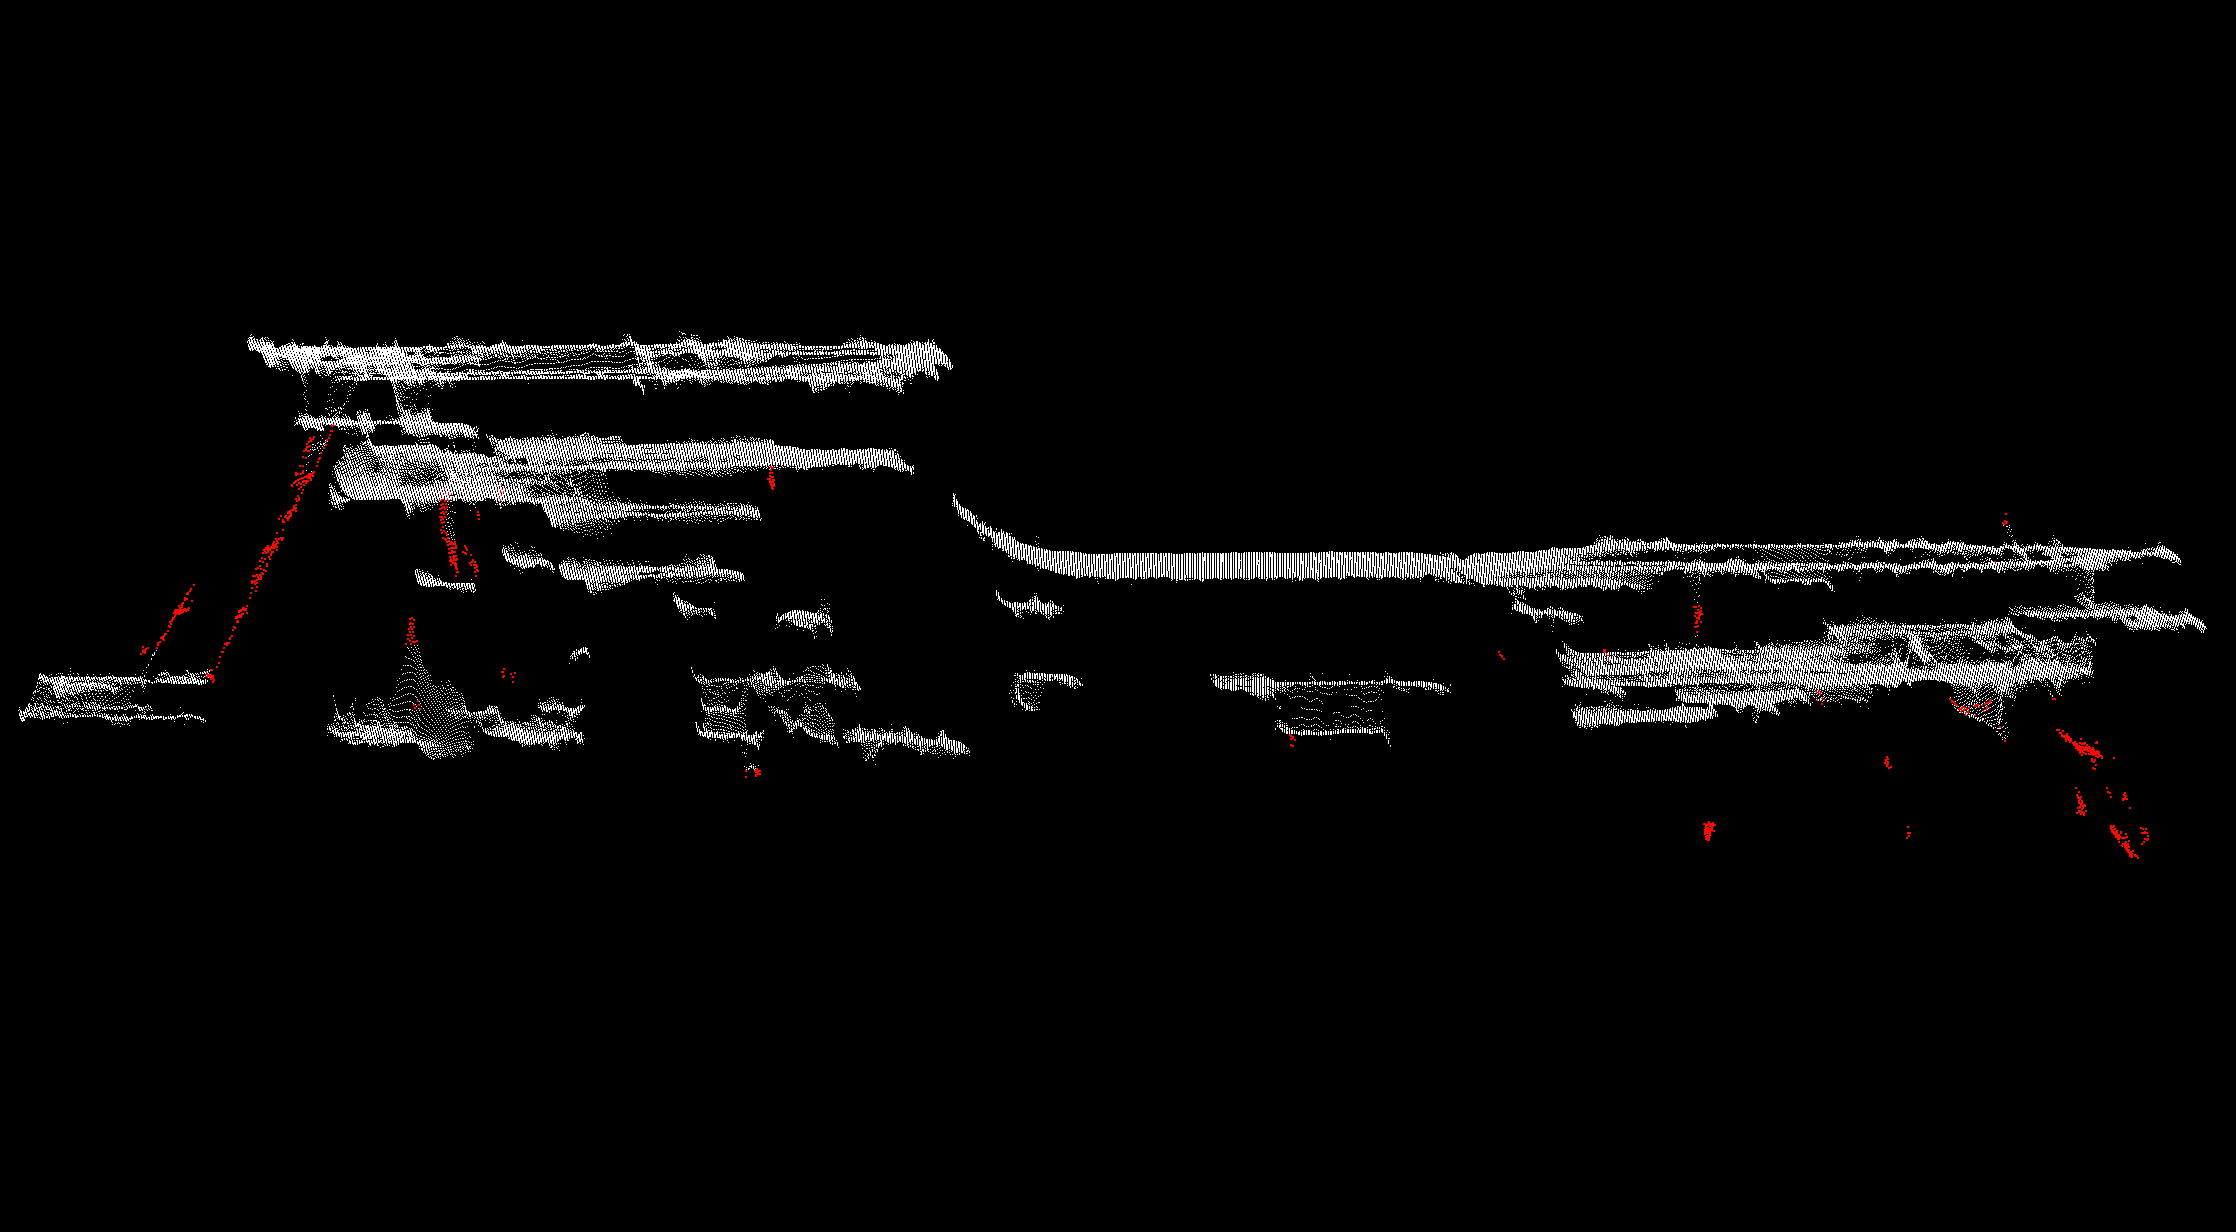
\includegraphics[width=0.75\textwidth]{figures/statistic.png}
    \caption{统计滤波侧视图}
    \label{fig:statistic}
\end{figure}

值得一提的是,对于一些结构简单,特征明显的物体,例如正常样本为平整表面的被检物,统计滤波算法可以直接用于对其进行缺陷检测。由于本文聚焦的是更为复杂的非平整表面,无法直接通过统计滤波实现理想的缺陷检测,但通过统计滤波能有效减少噪点,提升后续缺陷检测任务的准确性和效率,因此统计滤波只作为本文缺陷检测任务中点云预处理的一部分。


\subsection{点云下采样}
通常来说,结构光相机采集的点云数据非常庞大,以本文使用的梅卡曼德相机来说,其分辨率为$1920 \times1200$ ,每个点云数据点数约有两百万个点,单个点云存储文件约二十兆。即使经过前述直通滤波和统计滤波,提取出的ROI低噪声点云仍然有约三十万个点。稠密的原始点云能有效表现被摄物细节,但随之而来的是后续任务巨大的计算量。特别在工业生产环境下,时间就是金钱,企业不仅追求缺陷检测的算法性能,还同样关注算法的效率。

实际上在这些原始稠密点云中,有些点对于特征表现的贡献很小却依然会被计算。因此需要通过点云下采样在保留原始点云重要几何特征的同时减少点云中的点数,从而缩小点云整体规模,提升后续算法的计算效率。

点云下采样有不同的方法,例如随机,均匀或基于网格。本文采用基于网格的体素滤波进行下采样。体素滤波是一种对点云进行下采样的方法,它把三维空间划分成多个小立方体,然后用每个立方体的中心点或质心来近似该立方体内的所有点。
\begin{figure}[htbp]
    \centering
    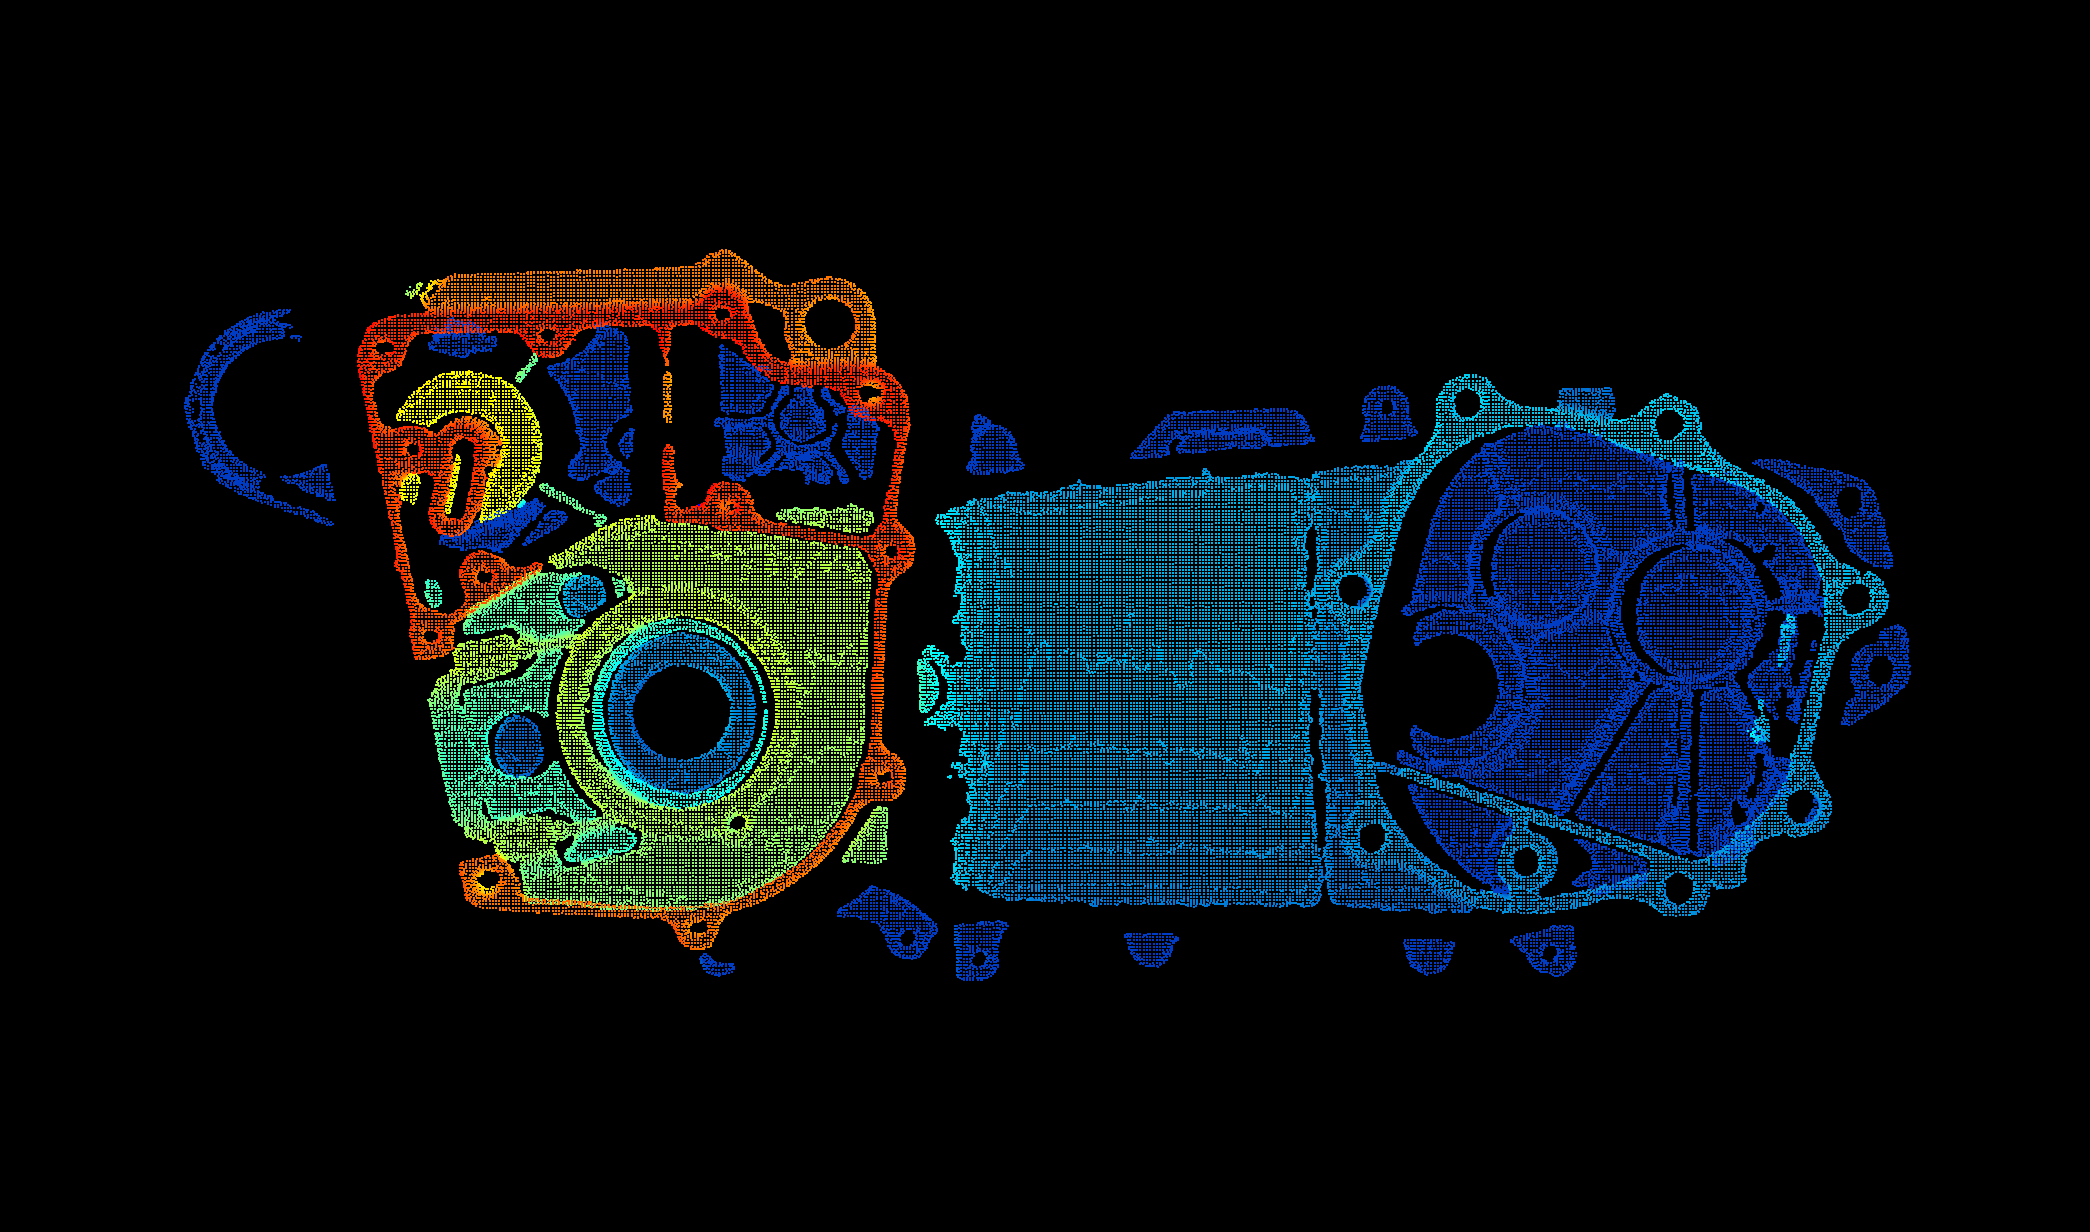
\includegraphics[width=0.75\textwidth]{figures/after_down.png}
    \caption{点云体素滤波效果图}
    \label{fig:aftet_down}
\end{figure}

网格大小是体素滤波的一个重要参数,网格太大,可能会导致原始点云的形状和特征丢失,甚至出现空洞和失真;网格太小,可能会导致下采样效果不明显。选择合适的网格大小才能既减少点云数据量,又保持原始点云的集合结构。本文经过多次实验选择0.001作为网格大小进行体素滤波,以采集的一个正常样本为例,体素滤波效果如图\ref{fig:aftet_down}所示。



\section{点云网格化}
\subsection{点云法线估计}
表面法线是在给定点垂直于表面的矢量。法向量表示表面的方向,可以用来提取对物体旋转和平移不变的特征。在点云和网格的情况下,可以通过计算每个点周围的局部几何来估计法向量。

估计一个点的法向量的最简单方法是使用最适合一小组相邻点的平面的表面法线。这被称为 PCA(主成分分析)方法,它涉及计算局部点云的协方差矩阵的特征向量。具有最小特征值的特征向量对应于局部表面的法向量。法线估计的效果如图\ref{fig:normal_estimation}所示,其中黑色箭头为估计的法向量。
\begin{figure}[htbp]
    \centering
    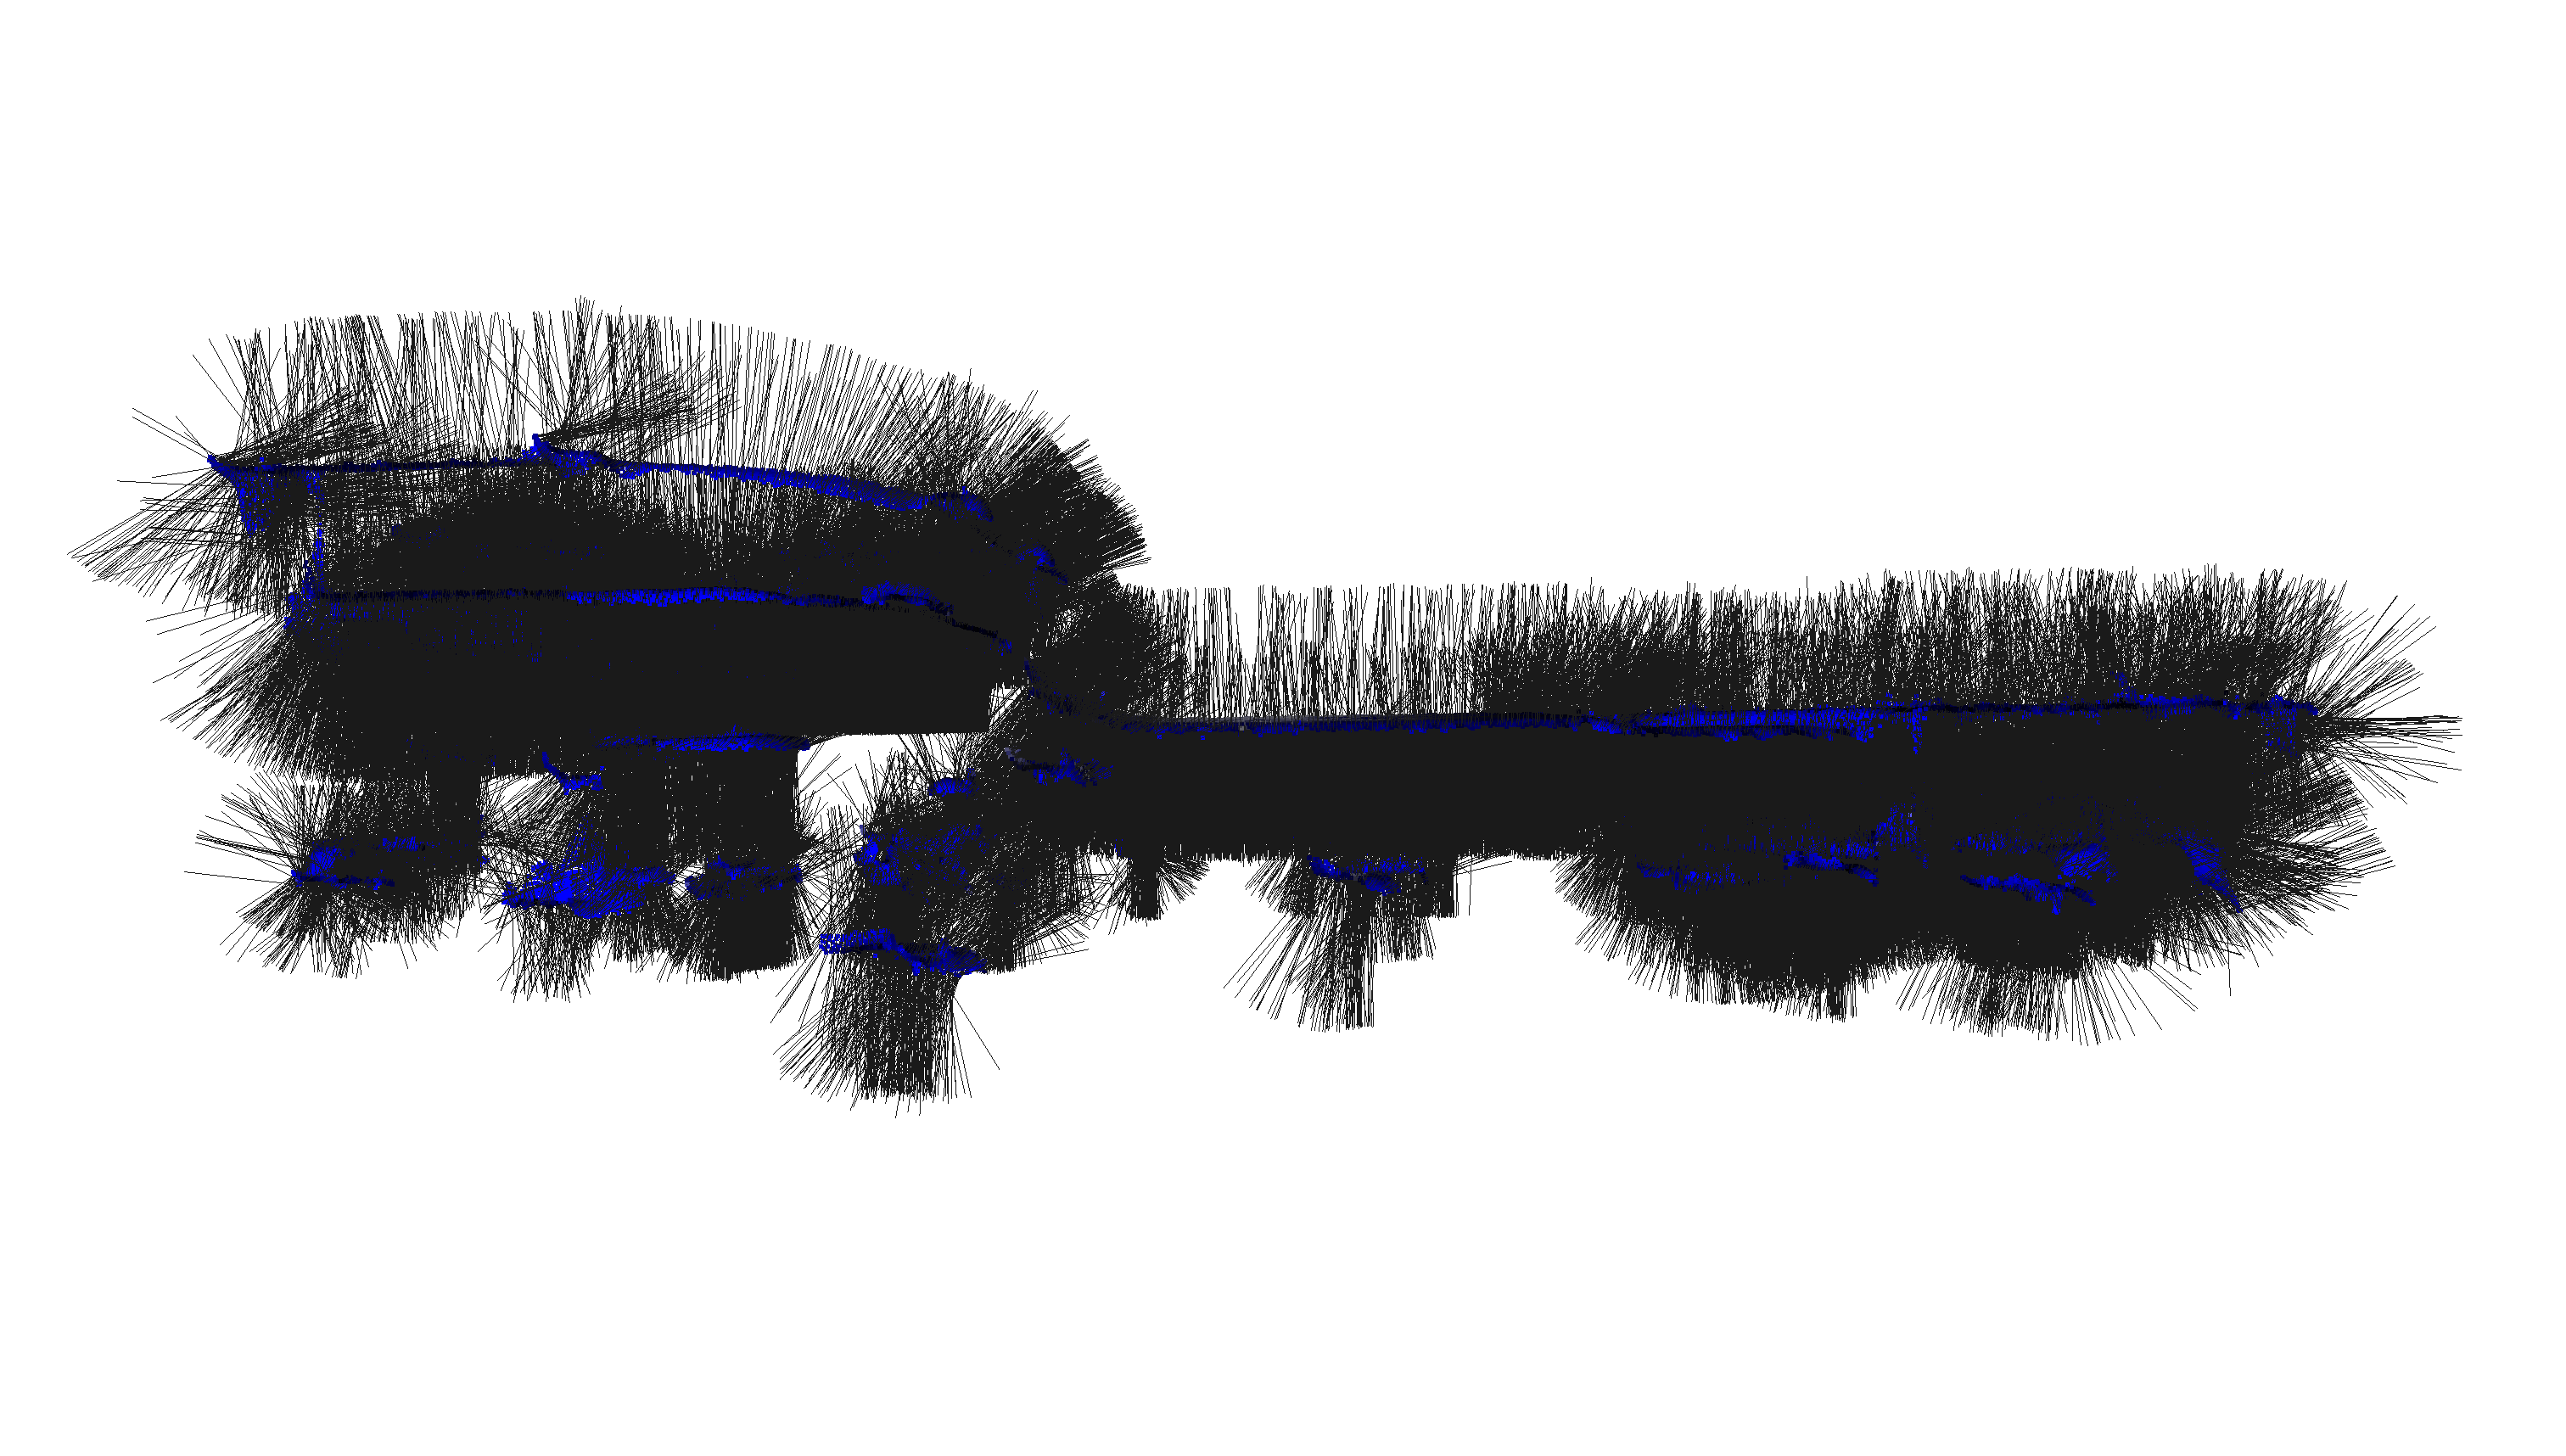
\includegraphics[width=0.75\textwidth]{figures/normal_estimation.png}
    \caption{法线估计侧视图}
    \label{fig:normal_estimation}
\end{figure}

\subsection{贪婪投影三角化}
Gopi等人\cite{gopiFastEfficientProjectionbased2002}使用贪婪投影三角网格化点云,其原理是维护一个点的列表,然后通过列表中的点不断延伸(即加入新的点)来构建网格,直到连接所有可能的点。其中三角剖分是面向局部的,先沿法线方向投影点的局部邻点,然后连接尚未连接的点以构建网格。
该算法基于增量表面生长原理,遵循贪婪方法。该算法从创建一个起始三角形开始,并不断添加新的三角形,直到覆盖所有点云中的点,或者没有更多可以加入到网格中的有效三角形。贪婪投影三角化的具体步骤如下:

第一步进行最近邻搜索,对于点云中的每个点 $p$,选择其k近邻。这个邻域通过搜索以参考点为球心、半径为$r$的球体中的最近k个邻点来定义。半径定为 $\mu .d$,其中$d$是点$p$到其最近邻点的距离,$\mu$是根据点云密度自定义的常数。通常使用Kdtree最近邻算法来寻找给定点的最近邻。

第二步进行切平面邻域投影,将邻域沿参考点$p$的法向量投影到与邻域形成的曲面近似相切的切平面上,并按角度排序。

第三步进行剪枝,按可视性和距离标准对邻域点进行剪枝,依次连接邻域点到参考点$p$和连续点,形成有最大角度约束和可选最小角度约束的三角形。其中遵循距离标准剪枝可以减少用Kdtree对当前点空间近似区域内候选邻接点的搜索。

\begin{table}[htbp]
    \centering
    \caption{贪婪投影三角化中点的类型} \label{tab:point-triangle}
    \begin{tabular*}{0.75\textwidth}{@{\extracolsep{\fill}}cc}
    \toprule
      类型&定义\\
      \midrule
      自由点&没有邻接三角形\\
      完成点	&所有邻接三角形都已确定\\
      边界点	&最大允许角度约束而缺失三角形的参考点\\
      边缘点	&尚未被选择作为参考点\\
    \bottomrule
    \end{tabular*}
\end{table}

可视性是用来排除可能产生自交网格的点。根据点在贪婪投影三角化算法中的状态,可以将其分为如表\ref{tab:point-triangle}所示的四种类型,在初始化时,点云中的点都是自由点。算法定义了两种边缘类型来检查可视性,一种是连接边缘点或边界点,只参与形成一个三角形边的边界边;另一种是连接完成点和其他点的内部边。使用参考点、候选点集以及边界边投影平面,如果从参考点到候选顶点的视线被边遮挡,则该点将被遮挡。

第四步是选择投影平面。将通过距离标准筛选的候选点集投影到近似切平面上,其中候选点为参考点为球心、半径为$r$球体内的所选点。

第五步是按角度排序。一个新的局部坐标系以参考点为坐标原点,以投影的平面为xy平面,所有候选点集中的点都被投影到该平面。候选点的角度是指局部坐标系x轴和从原点到投影后的候选点的向量间的夹角,并基于该角度进行排序。

按照上述步骤对点云进行贪婪投影三角化的效果如图\ref{fig:triangle}所示。

\begin{figure}[htbp]
    \centering
    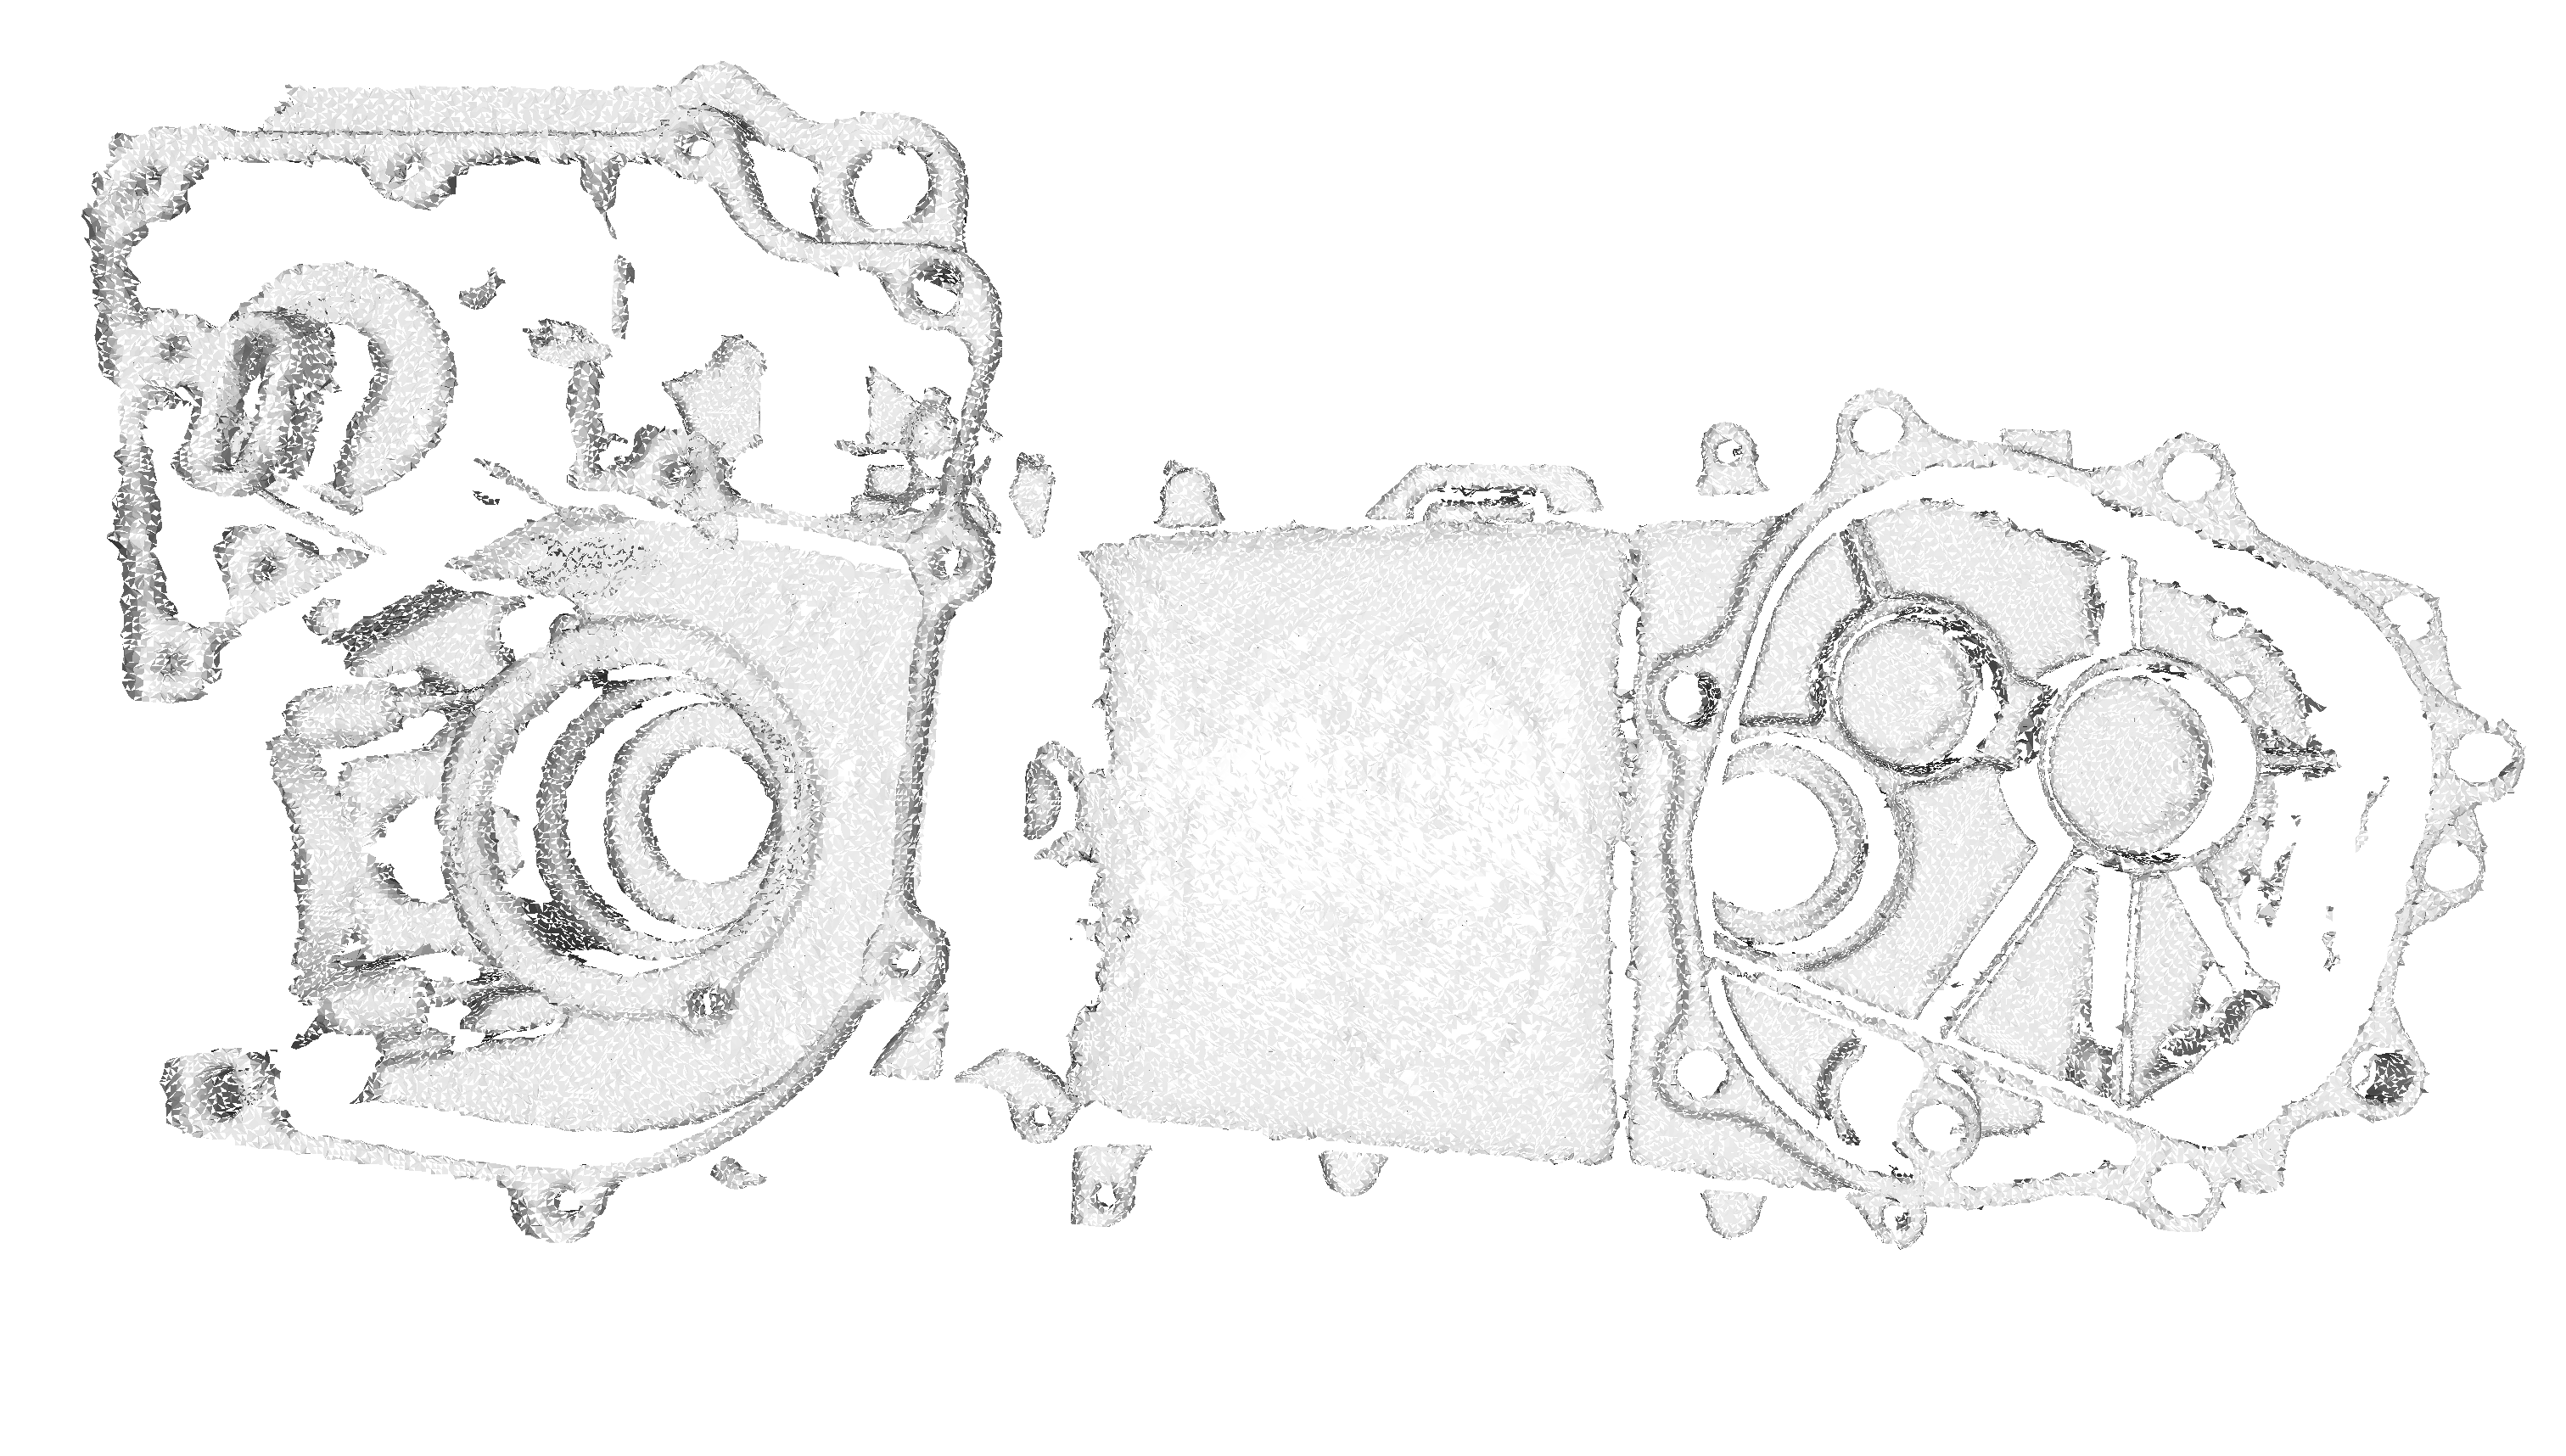
\includegraphics[width=0.75\textwidth]{figures/triangle.png}
    \caption{点云三角网格化}
    \label{fig:triangle}
\end{figure}

\section{点云局部特征提取}
RoPS\cite{yulanguoRoPSLocalFeature2013}是基于空间分布直方图的描述子,其构建的LRF(local reference frame)是独特且可重复的。RoPS算法包含两个部分。 首先,为每个关键点构造一个 LRF,并将局部表面与 LRF 对齐,以实现对刚性变换的不变性。 然后局部表面上的点分别绕三个坐标轴(即 x、y 和 z)旋转。 对于每次旋转,支撑区域中的点进一步投影到三个坐标平面(即 xy、yz 和 xz)上。

通过将平面划分为几个区间(bin)并计算落入每个区间的点数,为每个平面生成一个分布矩阵。 随后用五个统计量对分布矩阵进行编码。最后,通过连接所有旋转和投影的所有这些统计数据生成 RoPS 描述子。 RoPS 描述符的维度是$3\times3\times5\times drops_{r}$,其中 $drops_{r}$ 是围绕每个轴的旋转数。

\subsection{局部参考系LRF}

给定一个特征点p和支持半径r,在支持半径内包含N个三角形和M个顶点的局部表面网格S。对于其中第i个有$\symbfit{p}_{i1}$,$\symbfit{p}_{i2}$和$\symbfit{p}_{i3}$顶点的三角形。任意该三角形里的点可以通过式\ref{equ:point}表示,其中 $0 \leq s, t \leq 1$ 且$s+t \leq 1$。


\begin{equation}\label{equ:point}
    \symbfit{p}_{i}(s, t)=\symbfit{p}_{i 1}+s\left(\symbfit{p}_{i 2}-\symbfit{p}_{i 1}\right)+t\left(\symbfit{p}_{i 3}-\symbfit{p}_{i 1}\right)
\end{equation}

局部表面S的总协方差C定义为所有三角协方差矩阵的面积加权和。RoPS将特征点到三角形质心的距离作为新权重添加到协方差计算中,其作用是降低远处的点对总体协方差矩阵的贡献,减少郊区对矩阵的影响,从而进一步提高LRF对杂波和遮挡的鲁棒性。RoPS方法计算得到总协方差C的公式如式所示。

\begin{equation}
    \mathbf{C}=\sum_{i=1}^{N} w_{i 1} w_{i 2} \mathbf{C}_{i}
\end{equation}

其中N是局部表面S划分出的三角的数量,$\mathbf{C}_{i}$是第 $i$个三角的协方差矩阵,可由式\ref{equ:ci}计算而得。
\begin{equation}\label{equ:ci}
\begin{aligned}\mathbf{C}_{i} & =\int_{0}^{1} \int_{0}^{1-s}\left(\symbfit{p}_{i}(s, t)-\symbfit{p}\right)\left(\symbfit{p}_{i}(s, t)-\symbfit{p}\right)^{\mathrm{T}} d t d s \\& =\frac{1}{12} \sum_{j=1}^{3} \sum_{k=1}^{3}\left(\symbfit{p}_{i j}-\symbfit{p}\right)\left(\symbfit{p}_{i k}-\symbfit{p}\right)^{\mathrm{T}} \\& +\frac{1}{12} \sum_{j=1}^{3}\left(\symbfit{p}_{i j}-\symbfit{p}\right)\left(\symbfit{p}_{i j}-\symbfit{p}\right)^{\mathrm{T}}\end{aligned}
\end{equation}

此外, $w_{i1}$ 是第 $i$个三角面积和局部表面S的总面积,计算公式如下:

\begin{equation}
w_{i 1}=\frac{\left|\left(\symbfit{p}_{i 2}-\symbfit{p}_{i 1}\right) \times\left(\symbfit{p}_{i 3}-\symbfit{p}_{i 1}\right)\right|}{\sum_{i=1}^{N}\left|\left(\symbfit{p}_{i 2}-\symbfit{p}_{i 1}\right) \times\left(\symbfit{p}_{i 3}-\symbfit{p}_{i 1}\right)\right|},
\end{equation}

式中$\times$是叉乘。$w_{i 2}$与x特征点到第i个三角重心的距离有关,计算公式如下:

$$
w_{i 2}=\left(r-\left|\symbfit{p}-\frac{\symbfit{p}_{i 1}+\symbfit{p}_{i 2}+\symbfit{p}_{i 3}}{3}\right|\right)^{2} .
$$

然后,对加权协方差矩阵进行特征值分解(EVD)可以得到3个特征值大小依次递减的正交特征向量 $\left \{  \symbfit{v_{1}},\symbfit{v_{2}},\symbfit{v_{3}}\right \}$ 。但是这些向量的符号是有问题的,即使在同一网格的不同实例上也不可重复,因此需要重新定位每个特征向量的符号来消除符号模糊性。 $\symbfit{v_{1}}$的符号由式\ref{equ:3-sign}定义。

\begin{equation}\label{equ:3-sign}
    g=\operatorname{sign}\left(\sum_{i=1}^{N} w_{i 1} w_{i 2}\left(\frac{1}{6} \sum_{j=1}^{3}\left(\symbfit{p}_{i j}-\symbfit{p}\right) \symbfit{v}_{1}\right)\right)
\end{equation}

式中$\operatorname{sign}\left(\cdot\right)$表示提取实数符号的符号函数。以此类推可得 $\symbfit{v_{1}}$的符号, $\symbfit{v_{2}}$的符号则通过 $\symbfit{v_{3}} \times \symbfit{v_{1}}$得到。

因此,通过将 $\symbfit{p}$ 作为原点并分别使用 $\symbfit{v_{1}}$、$\symbfit{v_{2}}$和$\symbfit{v_{3}}$作为 $x$、 $y$和 $z$轴,最终定义了特征点 $\symbfit{p}$ 的唯一且可重复的3D局部参考框架。RoPS方法认为利用该LRF可以生成独特的、姿态不变的且具有高度区分性的局部特征描述符。

\subsection{局部特征描述子构造}

给定一个特征点及对应的LRF,通过将支持半径r里的所有相邻点的坐标$\mathrm {Q} = \left \{ q_{1},q_{2},... q_{M} \right \}$转换到LRF下来获得姿态不变性。转换后的点云定义为$\mathrm {Q'} = \left \{ q'_{1},q'_{2},... q'_{M} \right \}$ 。创建RoPS特征描述子的具体步骤如下:

首先,点云$\mathrm{Q'}$绕$x$轴旋转 $\theta_{k}$,旋转后的点云记为$\mathrm{Q'}\left(\theta_{k}\right)$。然后将$\mathrm{Q'}\left(\theta_{k}\right)$投影到 $xy$ 平面,生成的2D投影点云记为$\tilde{\mathrm {Q'}} \left ( \theta_{k}  \right )$ 。很明显,$\tilde{\mathrm {Q'}} \left ( \theta_{k}  \right )$ 提供了$\theta_{k}$视角下局部表面的一些独特信息。

接着,获得2D投影点云$\tilde{\mathrm {Q'}} \left ( \theta_{k}  \right )$ 的2D边界矩形,然后将其均匀地离散为$L\times L$区间。对落入每个区间中的点进行计数,统计成一个分布矩阵 $\mathrm{D}$。为了获得对不同网格分辨率的鲁棒性,还需对分布矩阵 $\mathrm{D}$进行归一化,即使所有区间之和为1。

RoPS使用矩理论将分布矩阵 $\mathrm{D}$的信息编码为紧凑有效的特征描述子,该理论因其数学简单和实用灵活,常被用于二维图像分析领域。给定一个矩阵 $\mathrm{D}$, $m+n$阶的中心距 $\mu_{mn}$定义如下:

\begin{equation}
    \mu_{m n}=\sum_{i=1}^{L} \sum_{j=1}^{L}(i-\bar{i})^{m}(j-\bar{j})^{n} \mathbf{D}(i, j)
\end{equation}

其中 $\bar{i}=\sum_{i=1}^{L} \sum_{j=1}^{L} i \mathbf{D}(i, j)$, $\bar{j}= \sum_{i=1}^{L} \sum_{j=1}^{L} j \mathbf{D}(i, j)$。

虽然理论上已经证明一个完整的矩集可以用来唯一地描述矩阵中包含的信息,但在实际应用时通常只有最有意义和最重要的矩子集被选择来表示矩阵。RoPS选择四个矩 $\left \{ \mu_{11},\mu_{12},\mu_{21},\mu_{22} \right \}$来形成特征描述子。

RoPS通过计算分布矩阵D的香农熵e并将其集成到特征描述子中来进一步增强特征描述子的描述性。其中香农熵e按式\ref{equ:3-e}定义。

\begin{equation}\label{equ:3-e}
    e=-\sum_{i=1}^{L} \sum_{j=1}^{L} \mathbf{D}(i, j) \log (\mathbf{D}(i, j))
\end{equation}


因此,来自$xy$平面的需要计算的统计量总共有五个,记为一个统计向量 $\left \{ \mu_{11},\mu_{12},\mu_{21},\mu_{22},e \right \}$。同样地,将旋转后的点云$\mathrm{Q'}\left(\theta_{k}\right)$投影到 $yz$和 $xz$平面,并且计算这两个平面对应的统计向量。

将来自$xy$、 $yz$和 $xz$平面的三个统计向量连接起来构成一个子特征 $f_{x} \left( \theta_{k}\right)$,用来描述原始点云绕 $x$轴旋转 $\theta_{k}$角度后的旋转点云的特征。当绕 $x$轴旋转角度的集合为 $\left \{ \theta_{1},\theta_{2},…,\theta_{T} \right \}$,对应的特征集合 $\left\{\symbfit{f}_{x}\left(\theta_{k}\right)\right\}, k=1,2, \ldots, T$。

为提升描述子描述性,点云除了围绕 $x$轴旋转生成的特征描述子,还以同样的方法绕 $y$轴旋转生成 $\left\{\symbfit{f}_{y}\left(\theta_{k}\right)\right\}, k=1,2, \ldots, T$和绕 $z$轴旋转生成 $\left\{\symbfit{f}_{z}\left(\theta_{k}\right)\right\}, k=1,2, \ldots, T$。最后,将绕 $x,y$和 $z$轴生成的三个子描述子合并到一个向量从而生成总特征描述子f,如式\ref{equ:rops-f}所示。 
\begin{equation}\label{equ:rops-f}
    \symbfit{f}=\left\{\symbfit{f}_{x}\left(\theta_{k}\right), \symbfit{f}_{y}\left(\theta_{k}\right), \symbfit{f}_{z}\left(\theta_{k}\right)\right\}, k=1,2, \cdots, T
\end{equation}

本文利用RoPS方法提取本章检测的金属件点云的3D局部特征,金属件上一个点的RoPS描述子如图\ref{fig:RoPS_and_histogram}所示。其中本文设置式\ref{equ:rops-f}中的T为3,因此RoPS特征直方图的维数为$3\times3\times5\times3 = 135$。

\begin{figure}[htbp]
    \centering
    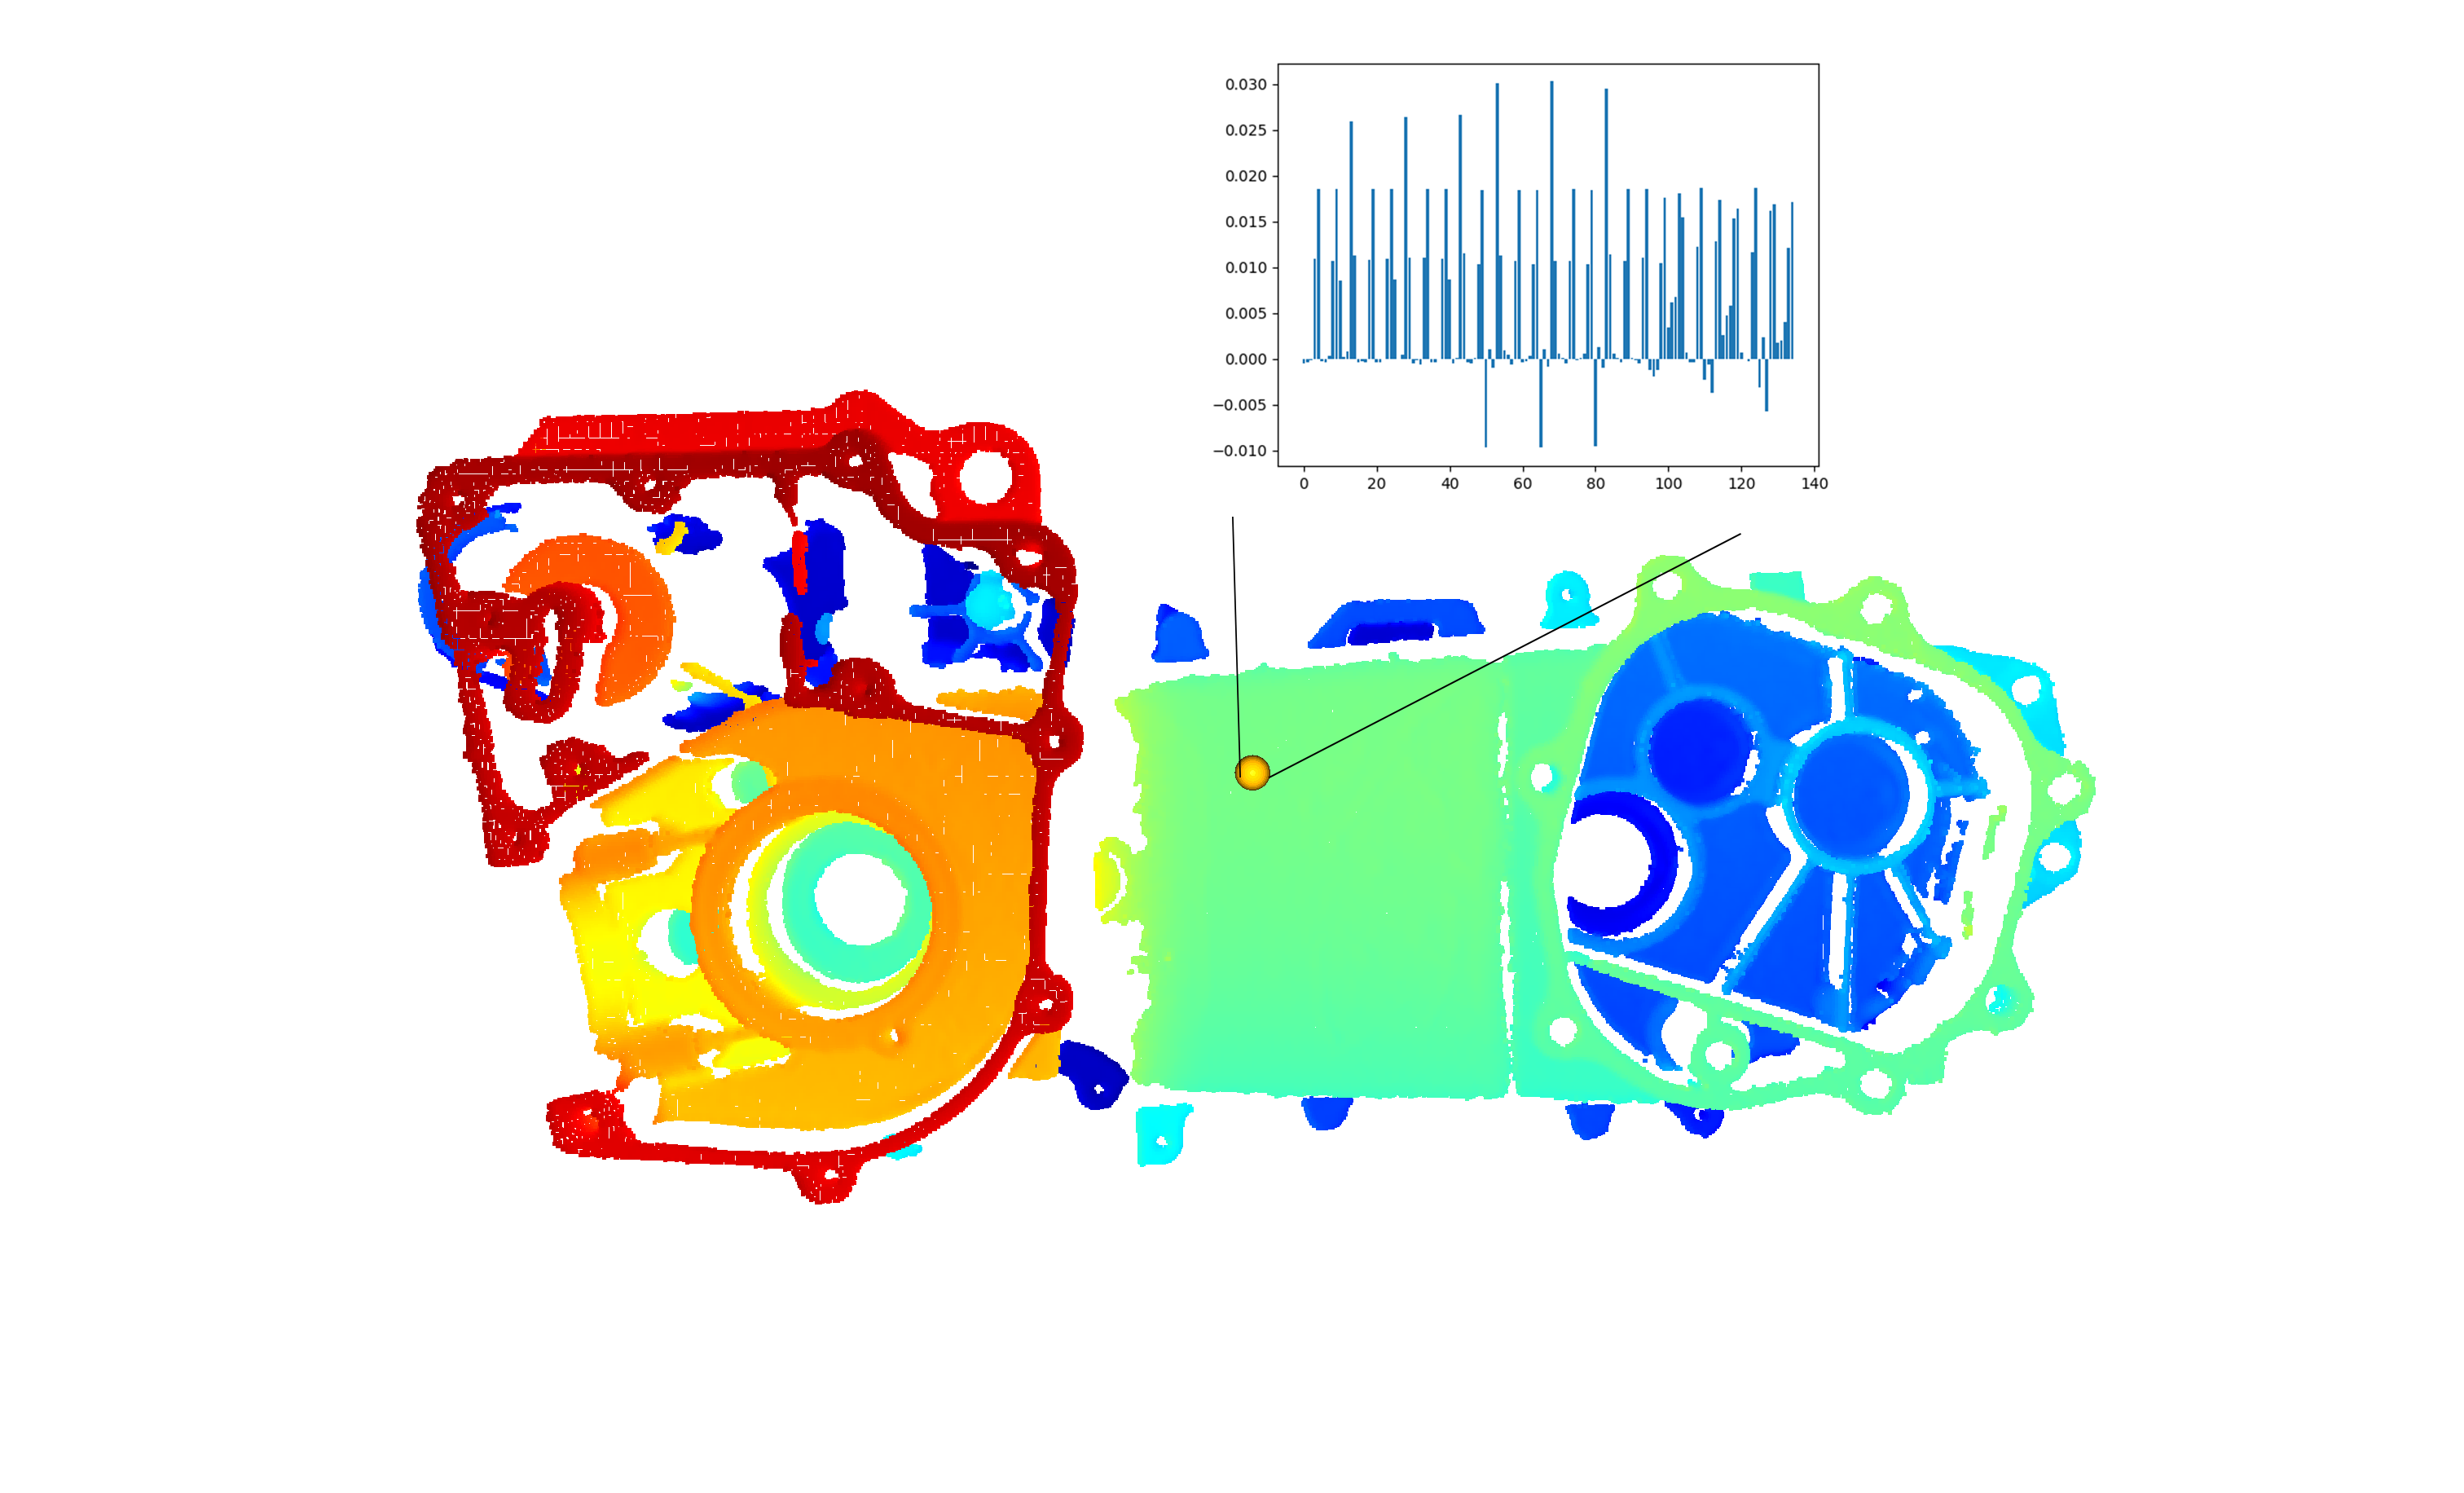
\includegraphics[width=1\textwidth]{figures/RoPS_and_histogram.png}
    \caption{RoPS描述子}
    \label{fig:RoPS_and_histogram}
\end{figure}

\section{三维缺陷检测}
PatchCore是应用在二维RGB图像上且表现出优异性能的无监督缺陷检测算法。PatchCore使用预训练网络对正常样本提取特征然后按块进行聚合到特征存储体并通过核心集降采样加快推理速度,最终通过测试数据的聚合特征与存储体最近邻距离输出异常得分。

本文通过结构光相机采集的点云数据实际上是2.5D数据,沿Z轴投影点云并经过插值等处理后即可生成深度图像,其通道为拍摄物到相机的距离。因此对于有序点云,经过标定对齐后,其x、y的值和其对应RGB图像的坐标一致,从而可以迁移PatchCore的方法,本文称基于PatchCore思想应用于点云的算法为PillarCore。
\subsection{柱特征}
本文用 $\mathcal{X}_{N}$定义所有训练时用的正常点云样本集 $\left(\forall x\in \mathcal{X}_{N}: y_{x}=0\right)$,用 $\mathcal{X}_{T}$定位测试时的点云样本集,用$y_{x} \in\{0,1\}$定义点云样本 $x$类型,其中(0)表示正常样本,(1)表示异常样本。类似于PatchCore将二维图像划分为块(Patch),本文的PillarCore将点云像切蛋糕一样划分为柱(Pillar)。

假设点云 $x_{i} \in \mathcal{X}$( $\mathcal{X}$为数据集)的特征 $\phi_{i} \in \mathbb{R}^{c^{*} \times h^{*} \times w^{*}}$是有 $c^{*}$ 深度$h^{*}$高度 $w^{*}$宽度的三维张量。用 $\phi_{i}(h, w)=\phi\left(x_{i}, h, w\right) \in \mathbb{R}^{c^{*}}$定义在位置 $h \in \{1,…,h^{*}\}$和 $w \in \{1,…,w^{*} \}$ 的$c^{*}$维RoPS特征描述子。

为了增加算法的鲁棒性同时不损失空间分辨率,在组成每个柱级特征表征时进行局部邻域聚合。来自邻域的特征向量按式\ref{equ:nphw} 定义 。

\begin{equation}\label{equ:nphw}
    \begin{aligned}\mathcal{N}_{p}^{(h, w)}=\{(a, b) \mid a & \in[h-\lfloor p / 2\rfloor, \ldots, h+\lfloor p / 2\rfloor], \\b & \in[w-\lfloor p / 2\rfloor, \ldots, w+\lfloor p / 2\rfloor]\},\end{aligned}
\end{equation}


在位置$(h,w)$的局部特征表示如式\ref{equ:aggf},其中$f_{\mathrm{agg}}$聚合邻域 $\mathcal{N}_{p}^{(h, w)}$里的特征向量。

\begin{equation}\label{equ:aggf}
    \phi_{i}\left(\mathcal{N}_{p}^{(h, w)}\right)=f_{\mathrm{agg}}\left(\left\{\phi_{i}(a, b) \mid(a, b) \in \mathcal{N}_{p}^{(h, w)}\right\}\right)
\end{equation}

对于特征张量 $\phi_{i}$,其局部特征集 $\mathcal{P}_{s, p}\left(\phi_{i}\right)$按式\ref{equ:localfeat}定义,其中步长参数 s 是可选的,一般设置为1。

\begin{equation}\label{equ:localfeat}
    \mathcal{P}_{s, p}\left(\phi_{i}\right)=\left\{\phi_{i}\left(\mathcal{N}_{p}^{(h, w)}\right) \mid\right.
 \left.h, w \bmod s=0, h<h^{*}, w<w^{*}, h, w \in \mathbb{N}\right\} 
\end{equation}

最后,对所有正常训练样本 $x_{i} \in \mathcal{X}_{N}$,本文参考PatchCore提出的块级特征存储体,针对点云数据建立了柱级特征存储体 $\mathcal{M}$,如式\ref{equ:memorybank} 所示。

\begin{equation}\label{equ:memorybank}
    \mathcal{M}=\bigcup_{x_{i} \in \mathcal{X}_{N}} \mathcal{P}_{s, p}\left(\phi_{j}\left(x_{i}\right)\right)
\end{equation}

\subsection{核心集降采样}
对持续增长的$\mathcal{X}_{N}$,$\mathcal{M}$变得非常大,因此评估新测试数据的推断时间和所需的存储量都会增加。随机二次抽样从一定程度上能解决问题,但几个数量级的抽样将丢失在正常样本特征覆盖范围内编码的$\mathcal{M}$中可用的重要信息。本文采用PatchCore提出的核心集降采样机制来减少$\mathcal{M}$ ,这样可以在保持性能的同时减少推理时间。

理论上,核心集选择的目的是找到子集 $\mathcal{S} \subset \mathcal{A}$,使得在A上的问题求解能最接近,特别是更快速地逼近在S上计算求解。根据具体问题,关注的核心集有所不同。Patchcore由于使用最近邻计算,其选择使用一种极小极大设施选址(minimax facility location) 算法进行核心集选择,如式\ref{equ:mdown}所示,来确保与原始存储体$\mathcal{M}$ 相比,$\mathcal{M}$ 的核心集$\mathcal{M}_c$ 在块级特征空间的覆盖率大致相似。

\begin{equation}\label{equ:mdown}
    \mathcal{M}_{C}^{*}=\underset{\mathcal{M}_{C} \subset \mathcal{M}}{\arg \min } \max _{m \in \mathcal{M}} \min _{n \in \mathcal{M}_{C}}\|m-n\|_{2} .
\end{equation}

$\mathcal{M}_{C}^{*}$的精确计算是NP-HARD问题。PatchCore使用迭代贪婪近似,来进一步减少核心集的选择时间。利用Johnson-Lindenstrauss定理,通过随机线性投影 $\psi: \mathbb{R}^{d} \rightarrow \mathbb{R}^{d^{*}}$   ,其中 $d^{*}<d$  来减少元素 $m \in \mathcal{M}$的维度。

% 存储体的降维总结为伪代码。


\subsection{缺陷检测}
建立正常样本块特征存储体后,PatchCore通过测试图像 $x^{test}$的块集合 $\mathcal{P}\left(x^{\text {test }}\right)=\mathcal{P}{s, p}\left(\phi{j}\left(x^{\text {test }}\right)\right)$中测试块特征和$\mathcal{M}$ 中的每个最近邻 $m^{*}$之间的最大距离分数 $s^{*}$,对测试图像 $x^{test}$估计图像级异常分数 $s \in \mathbb{R}$ 。其中$s^{*}$的计算公式如式\ref{equ:sstar}所示。

\begin{equation}\label{equ:sstar}
    \begin{aligned}m^{\text {test }, *}, m^{*} & =\underset{m^{\text {test }} \in \mathcal{P}\left(x^{\text {test })}\right)}{\arg \max } \underset{m \in \mathcal{M}}{\arg \min }\left\|m^{\text {test }}-m\right\|_{2} \\s^{*} & =\left\|m^{\text {test }, *}-m^{*}\right\|_{2} .\end{aligned}
\end{equation}


PatchCore通过使用$s^{*}$上的缩放因子w来表示相邻块的关系从而计算s,如式\ref{equ:score}所示。如果最接近异常候选 $m^{\text {test},* }$, $m^{*}$的存储体特征本身远离相邻样本,即很少出现的正常样本,缩放因子会使异常分数增加。

\begin{equation}\label{equ:score}
    s=\left(1-\frac{\exp \left\|m^{\text {test }, *}-m^{*}\right\|_{2}}{\sum_{m \in \mathcal{N}_{b}\left(m^{*}\right)} \exp \left\|m^{\text {test }, *}-m\right\|_{2}}\right) \cdot s^{*}
\end{equation}

其中 $\mathcal{N}_{b}\left(m^{*}\right)$ 是$\mathcal{M}$ 中离测试块特征 $m^{*}$最近的b个块特征。这种重新加权比最大块距离更鲁棒。图像级异常的分需要通过对每个块进行arg max运算得出。此外,还可在同一步骤中计算分割图,通过基于他们各自空间位置调整计算的异常得分。

PatchCore的核心集降采样和异常得分计算都是在进行特征聚合后,而本文所研究的点云数据在经过柱特征抽象后与二维RGB图像块特征抽象后的表现形式相近,因此本文的PillarCore直接复用其后续流程方法,实现点云数据的缺陷检测。

\section{实验设计及结果分析}
\subsection{数据集}
本文被检对象为实验室的摩托车金属件,该金属件结构复杂,最小外接立方体的长宽高为$0.52m\times 0.22m \times 0.09m$,其XY方向点云标量图如图\ref{fig:pcdxy}所示。
\begin{figure}[htbp]
    \centering
    \begin{subfigure}
        \centering
        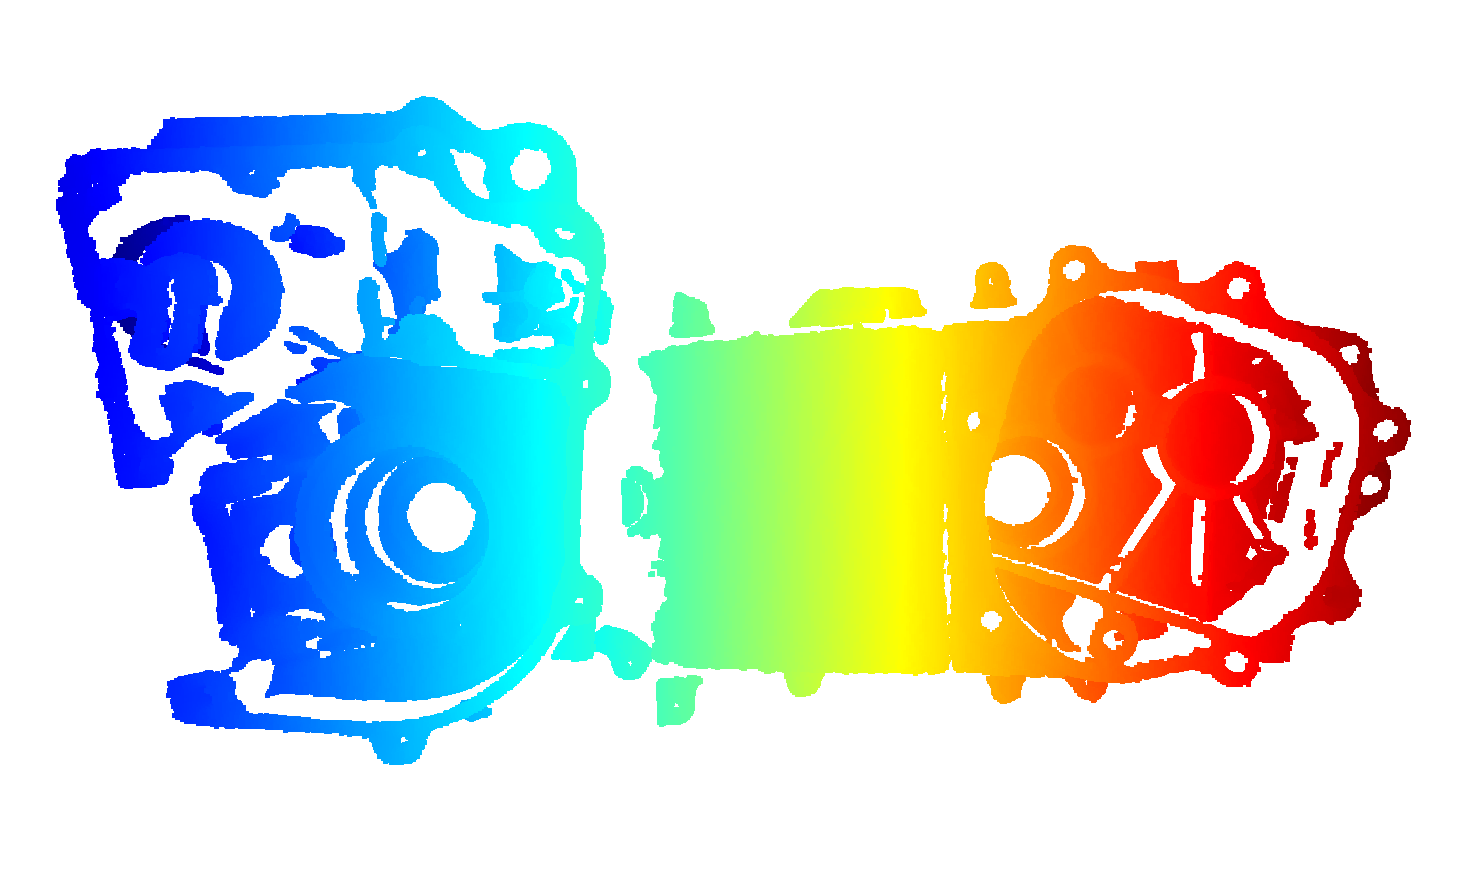
\includegraphics[width=.4\linewidth]{figures/3/normal-x.png}  
      \end{subfigure}
      \begin{subfigure}
        \centering
        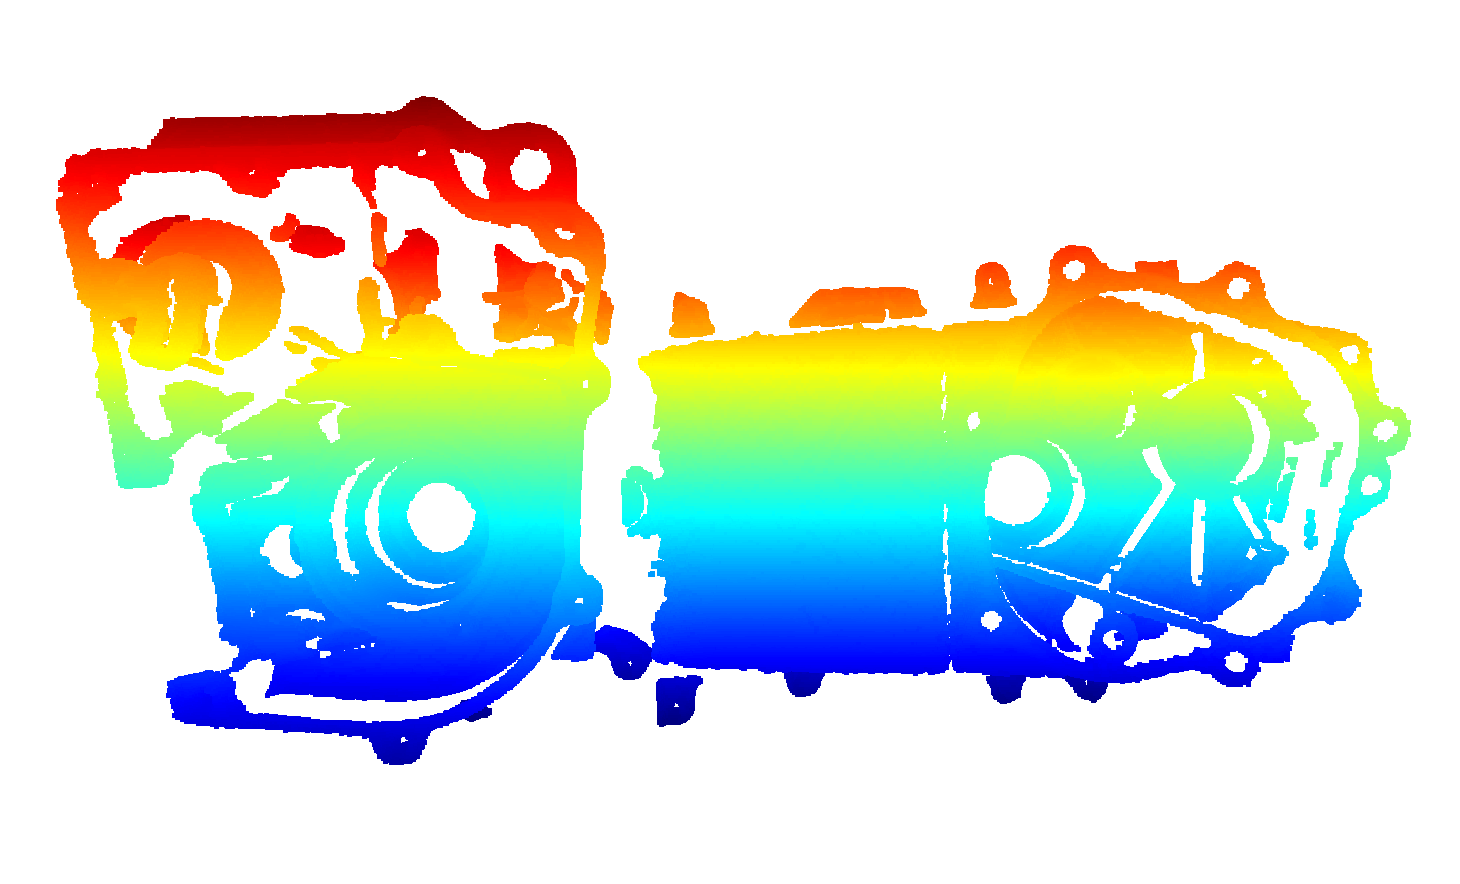
\includegraphics[width=.4\linewidth]{figures/3/normal-y.png} 
      \end{subfigure}
    \caption{采集点云数据XY标量图}
    \label{fig:pcdxy}
  \end{figure}

本文使用第二章搭建的实验平台对金属件进行拍摄,采集正常样本和手工制造的缺陷样本的点云数据制作数据集。其中训练数据集全部为正常样本,测试数据集由结构缺陷和正常样本共同组成。部分正常样本和缺陷样本如图\ref{fig:normalxy}和图\ref{fig:bad}所示。其中图\ref{fig:normalxy}中的正常样本是对同一工件从多个角度采集的。图\ref{fig:bad}中红色框表示缺陷样本缺陷处俯视和侧视两个角度的视图。侧视视角中,红框范围内绿色部分点云为缺陷样本中的一个结构缺陷。

  \begin{figure}[htbp]
    \centering
    \begin{subfigure}
        \centering
        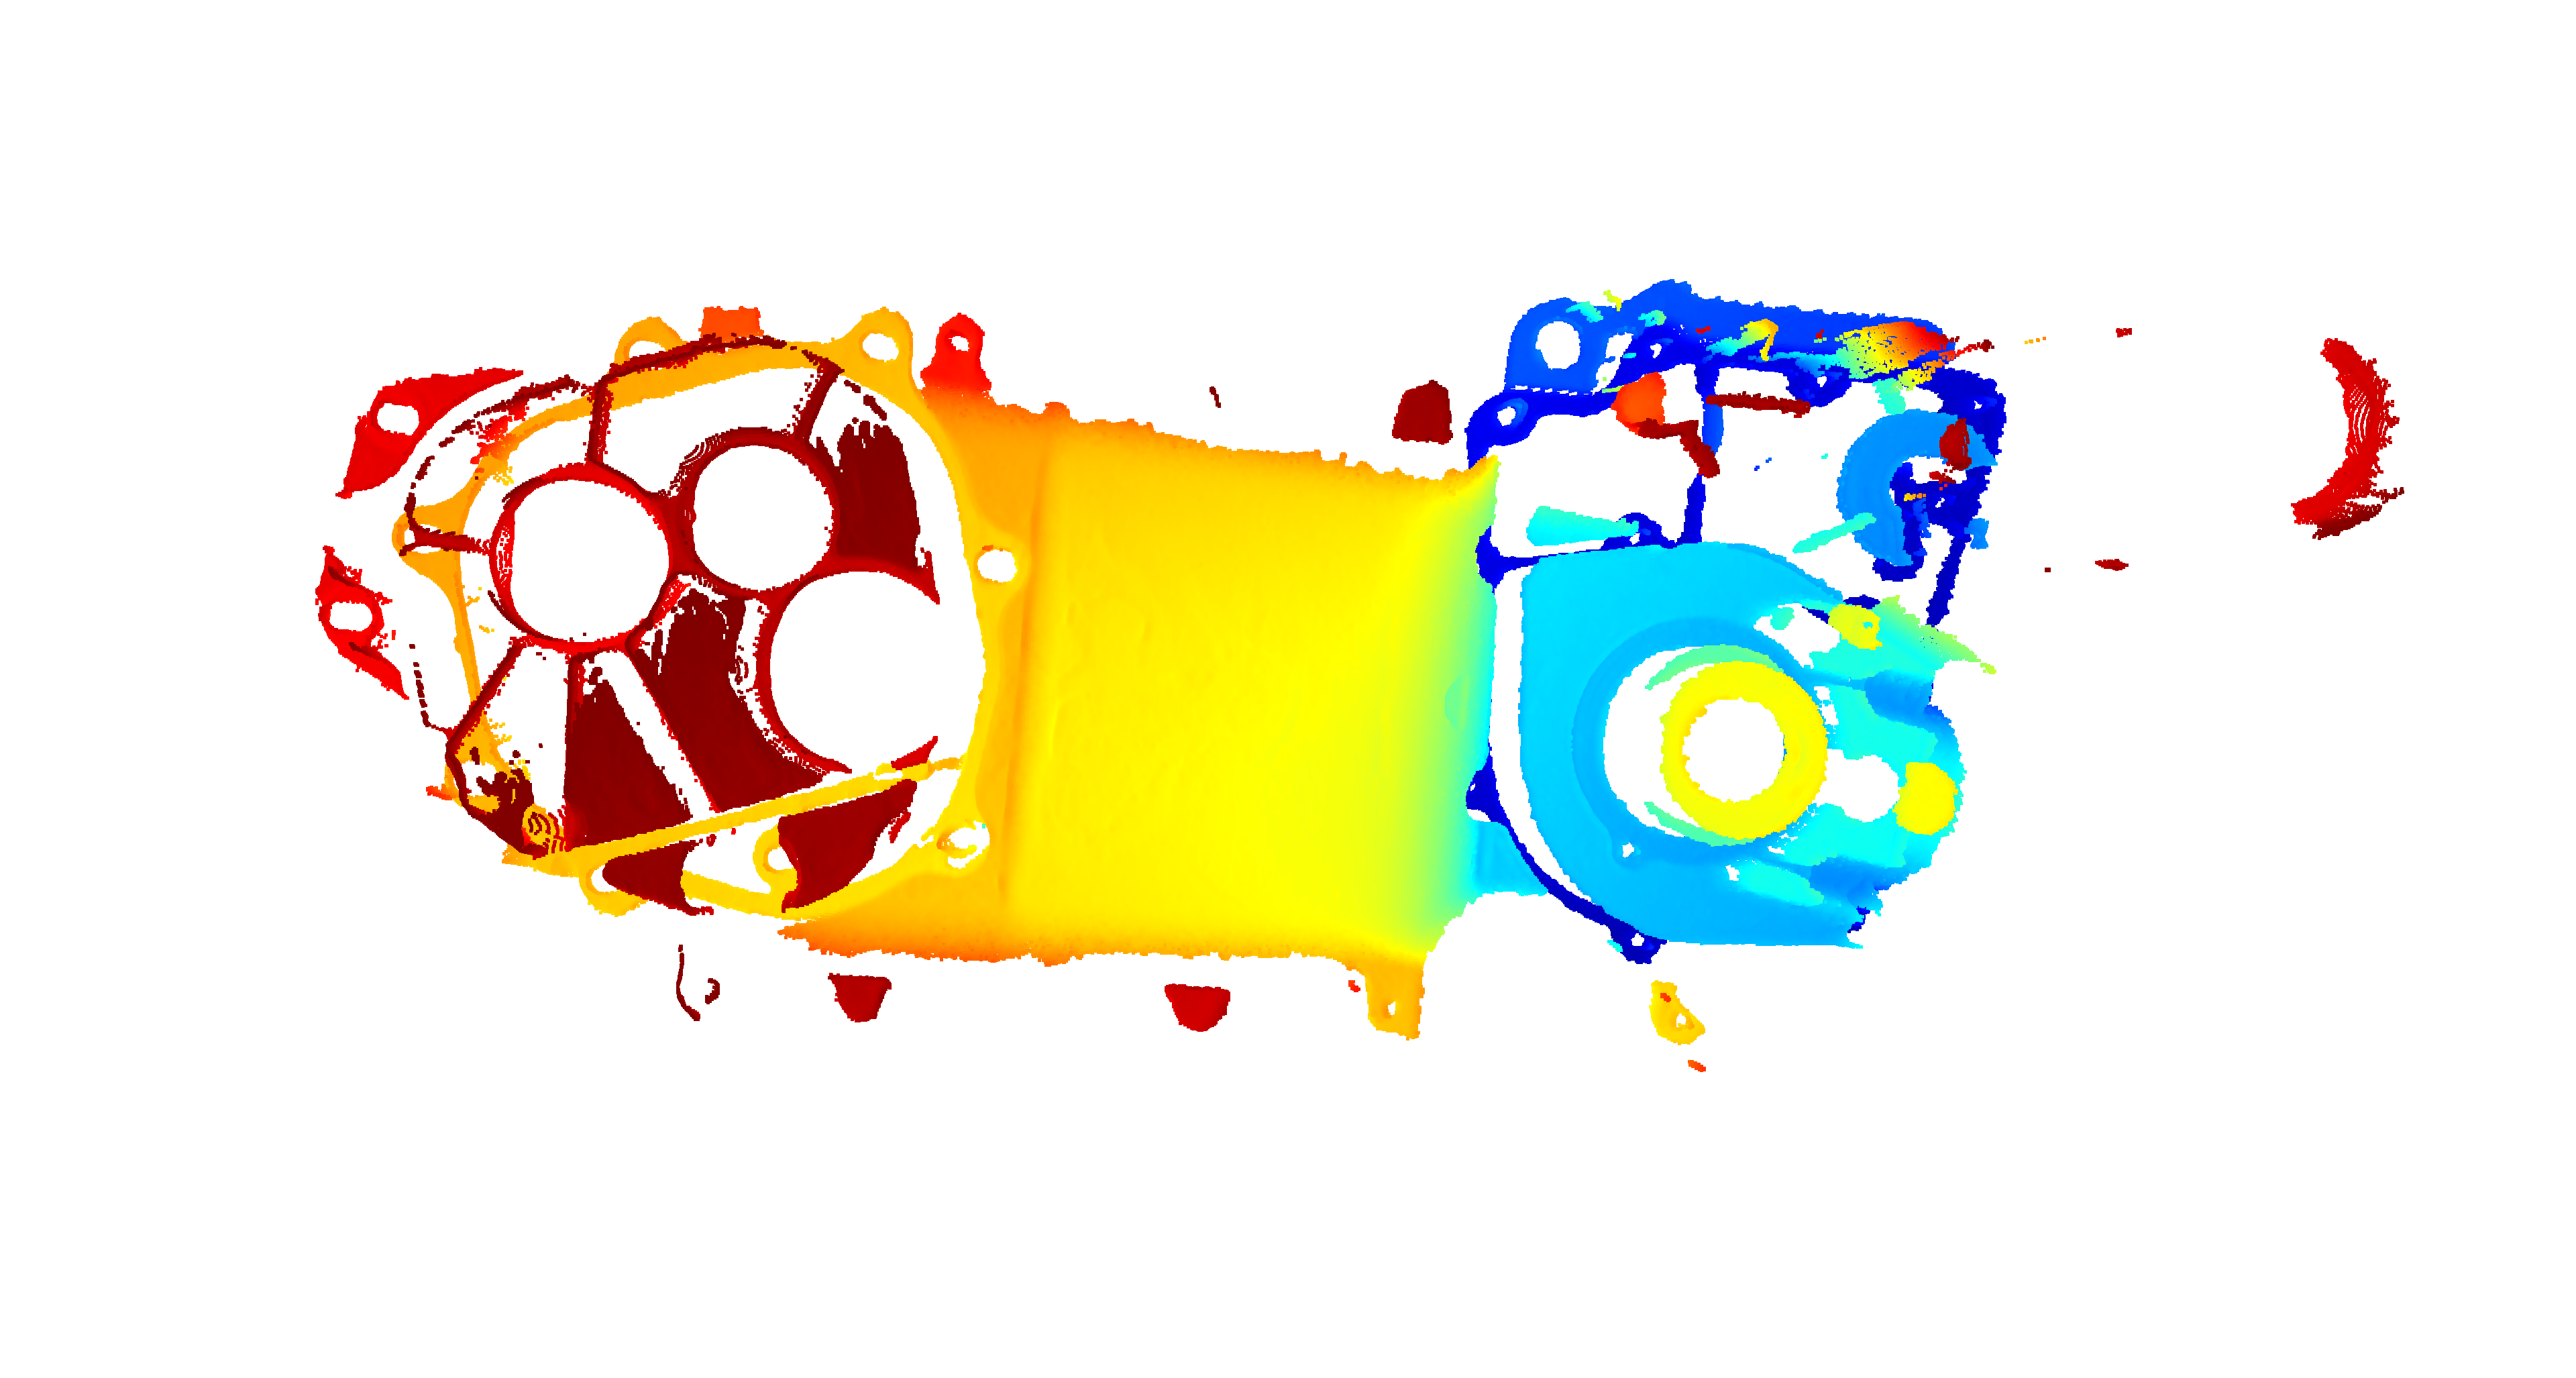
\includegraphics[width=.4\linewidth]{figures/3/good-1.png}  
      \end{subfigure}
      \begin{subfigure}
        \centering
        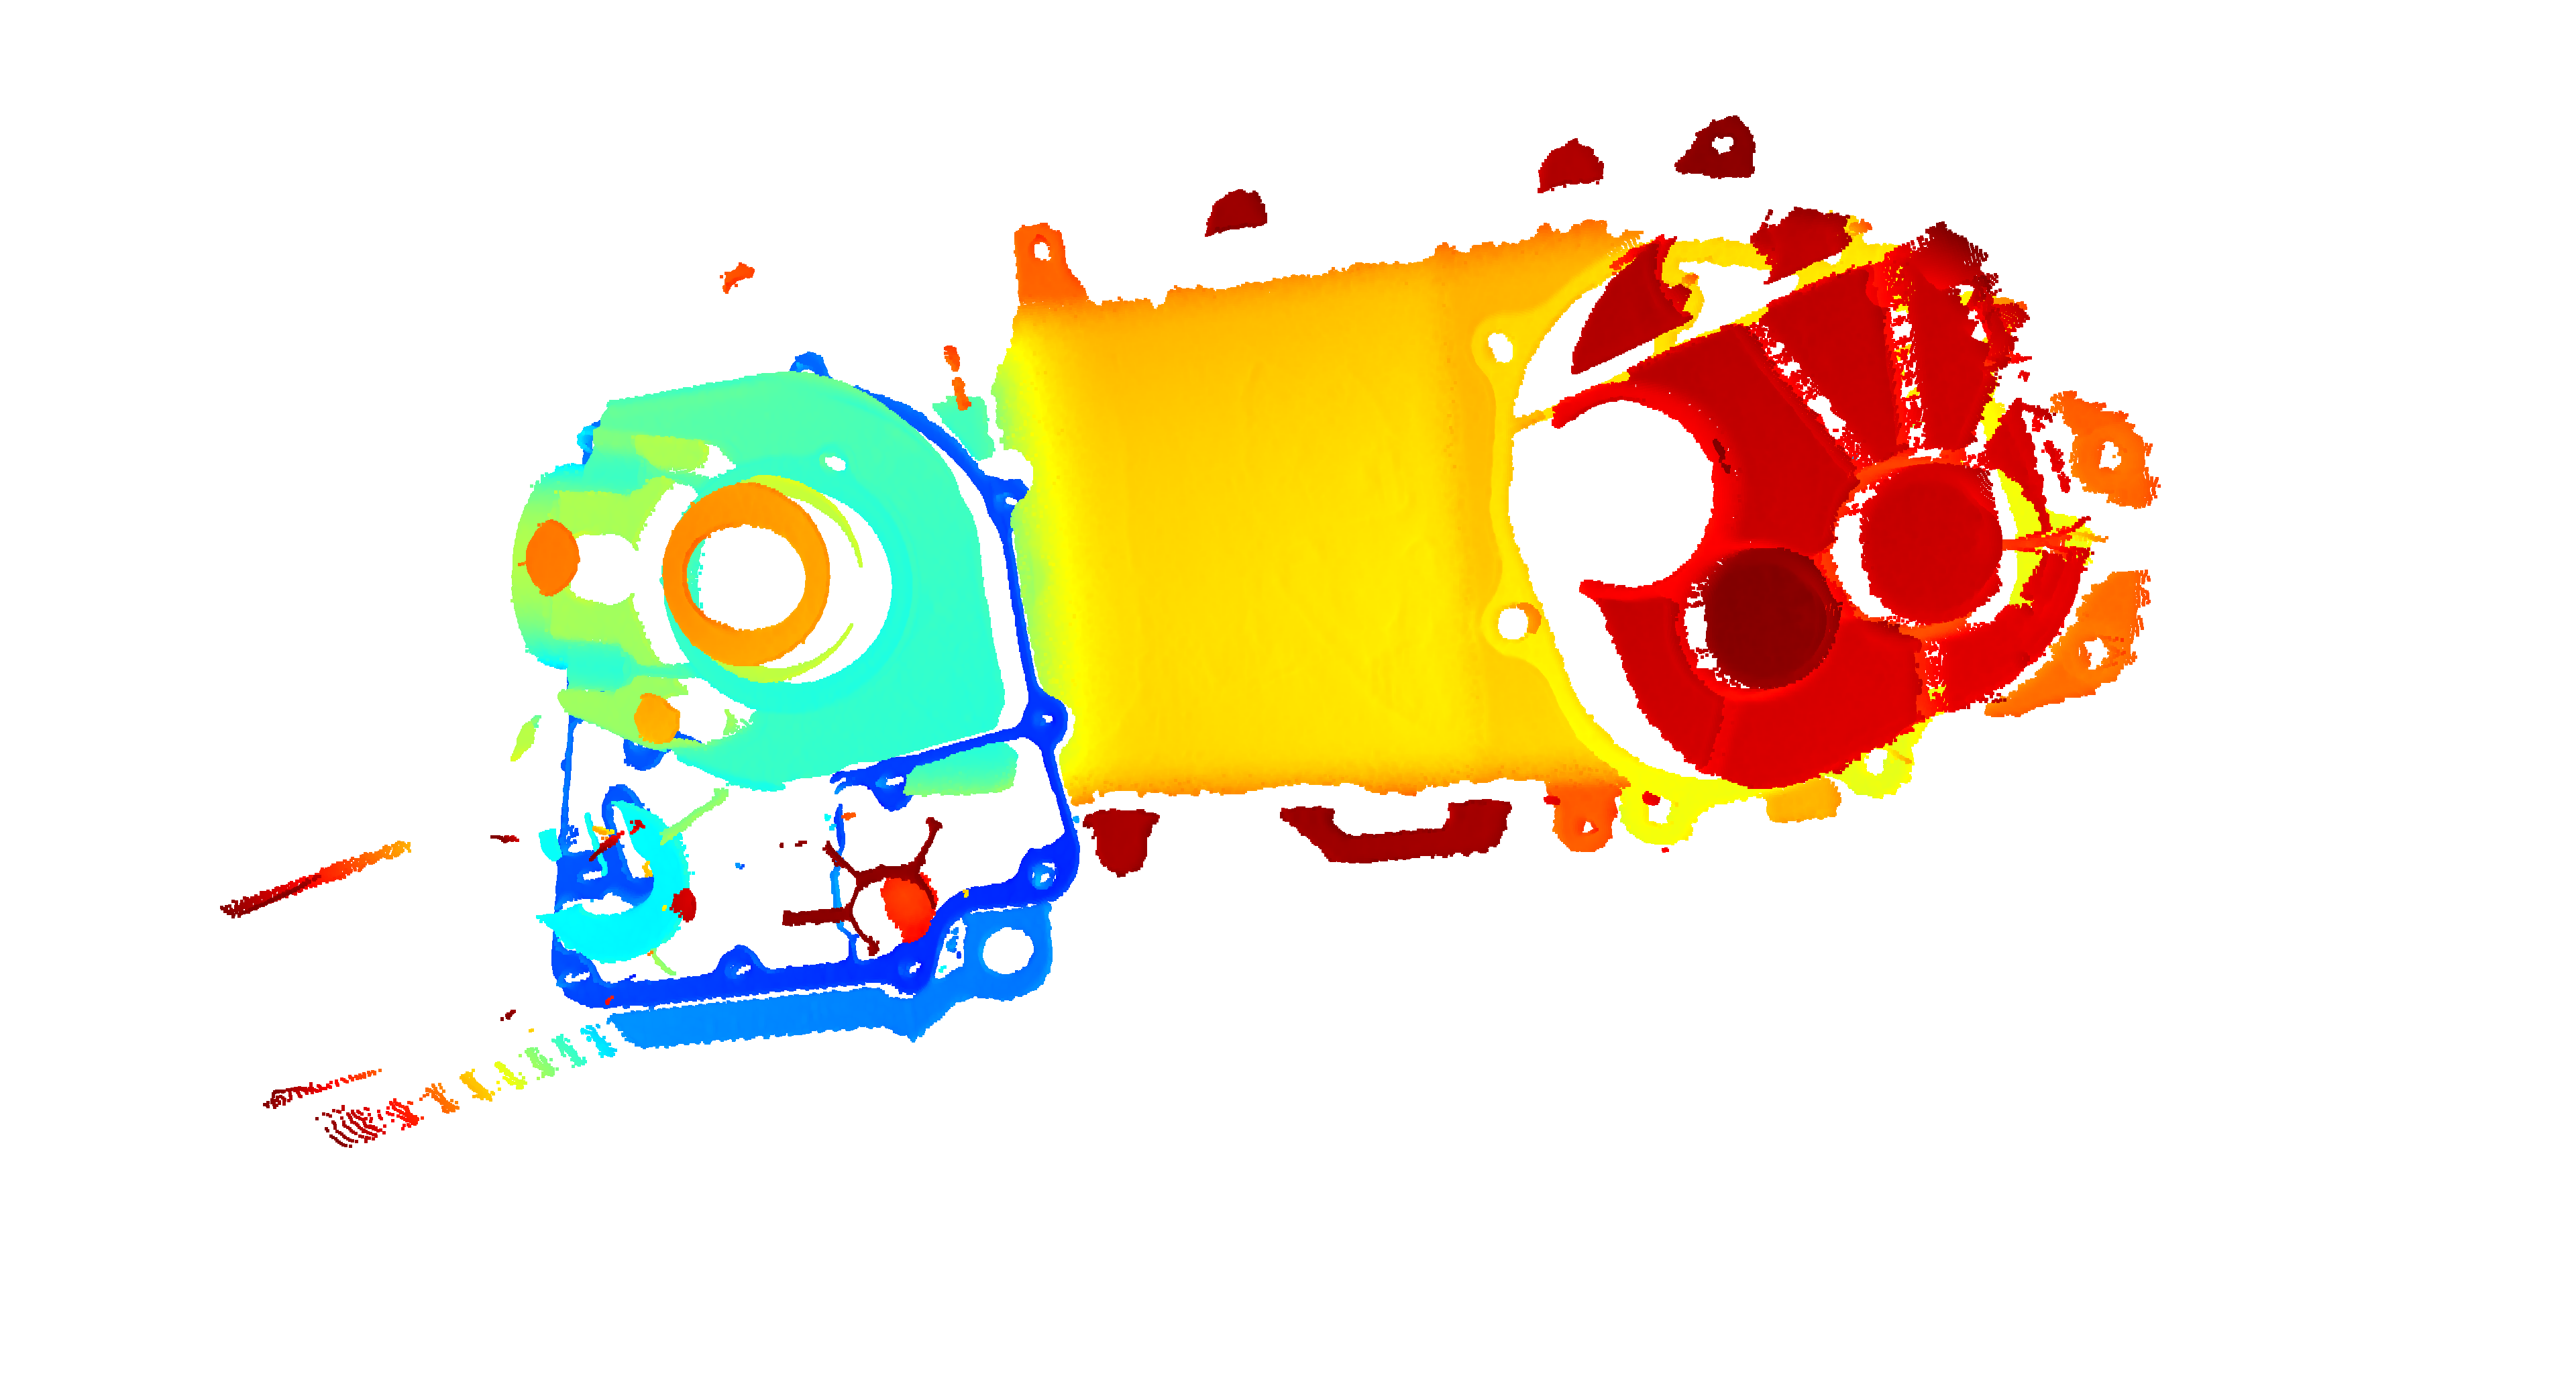
\includegraphics[width=.4\linewidth]{figures/3/good-2.png} 
      \end{subfigure}
      \begin{subfigure}
        \centering
        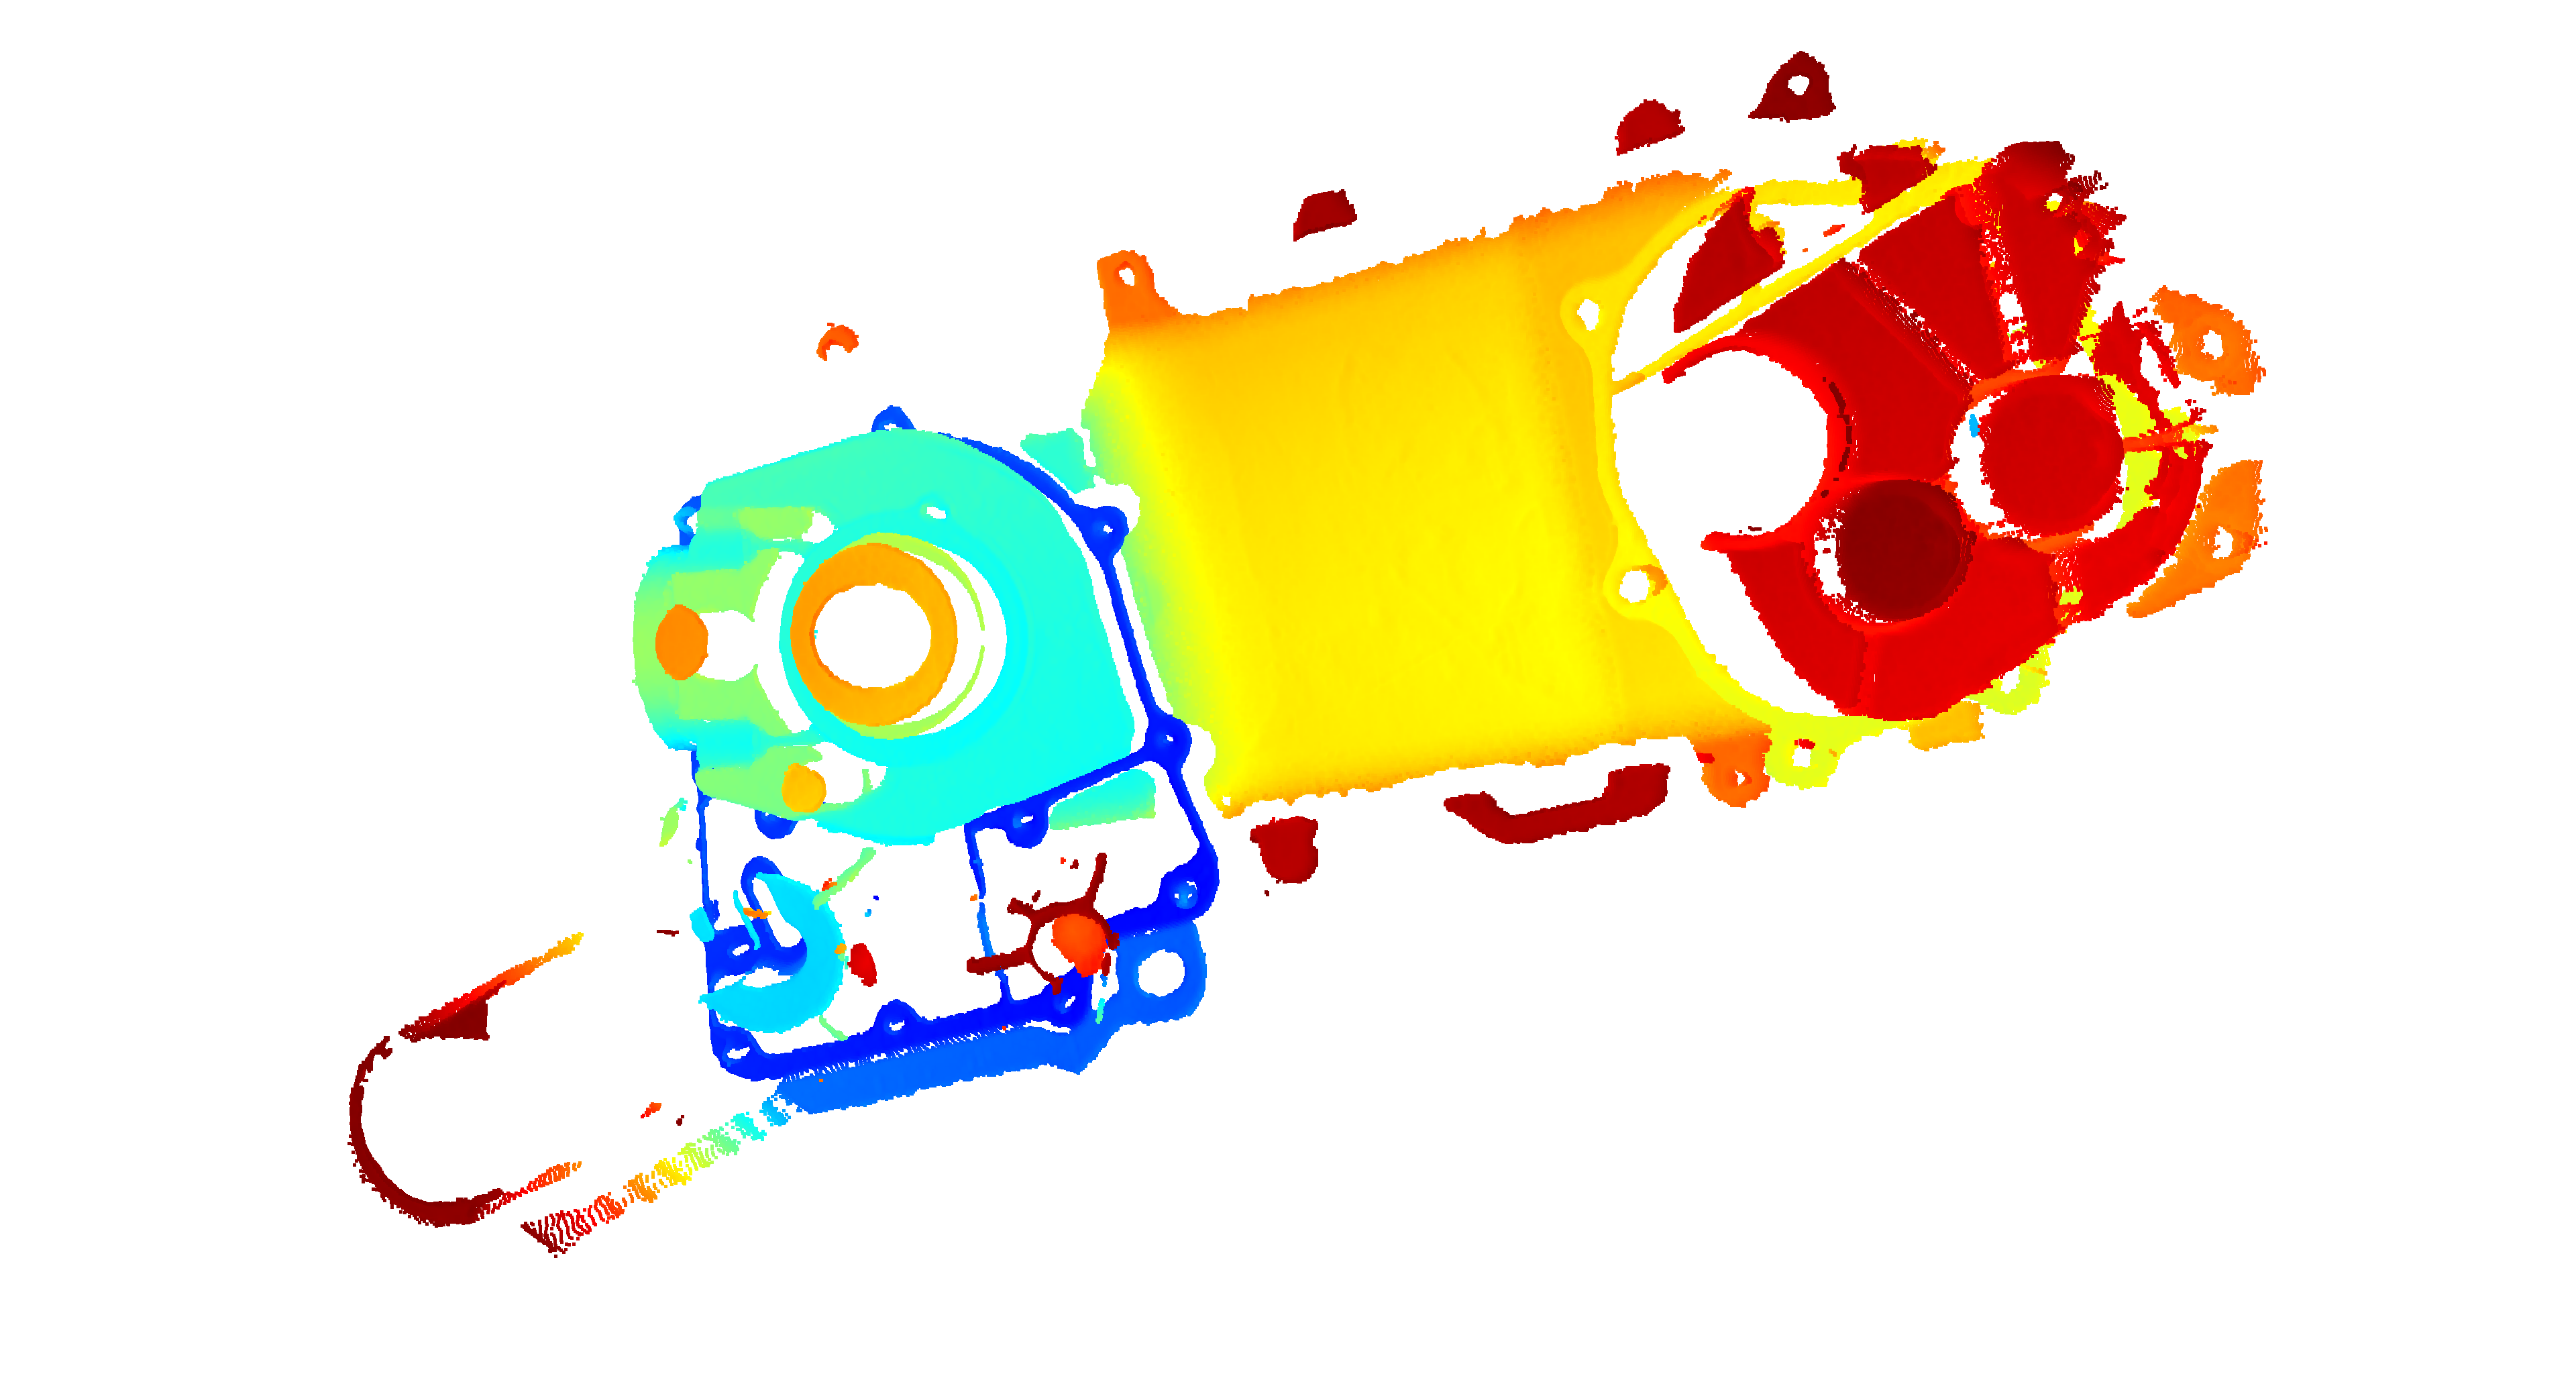
\includegraphics[width=.4\linewidth]{figures/3/good-3.png}  
      \end{subfigure}
      \begin{subfigure}
        \centering
        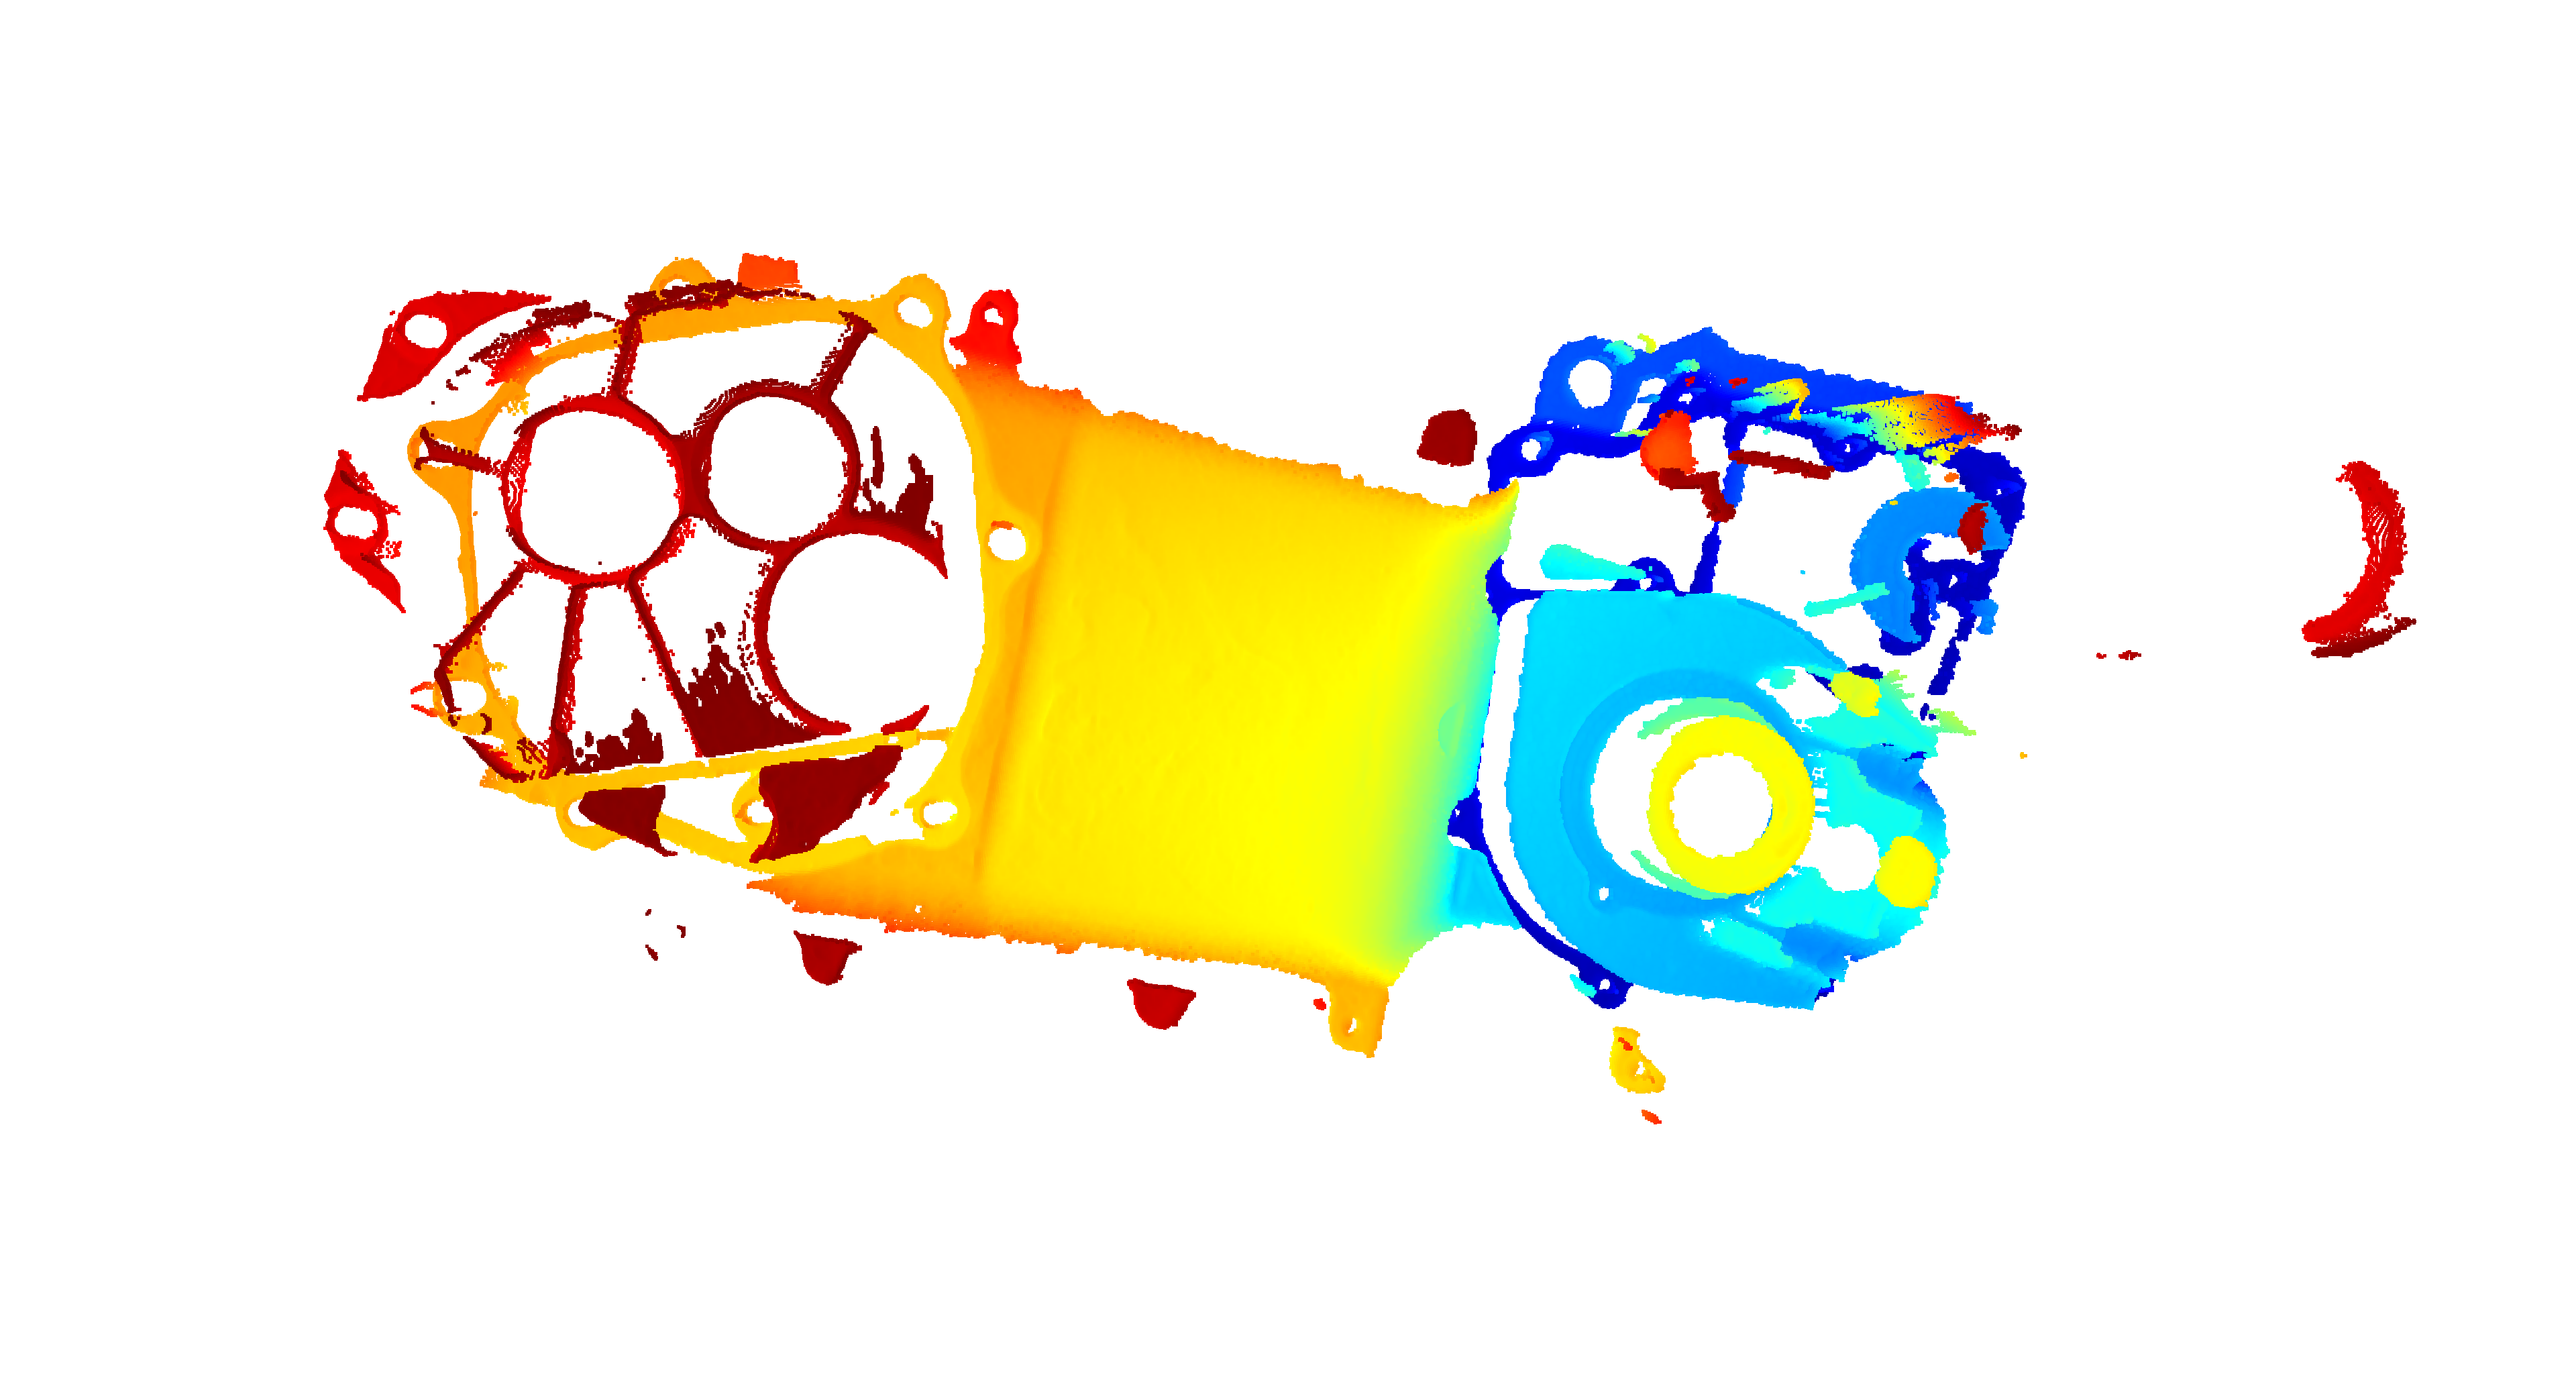
\includegraphics[width=.4\linewidth]{figures/3/good-4.png} 
      \end{subfigure}
    \caption{部分正常样本}
    \label{fig:normalxy}
  \end{figure}

  \begin{figure}[htbp]
    \centering
    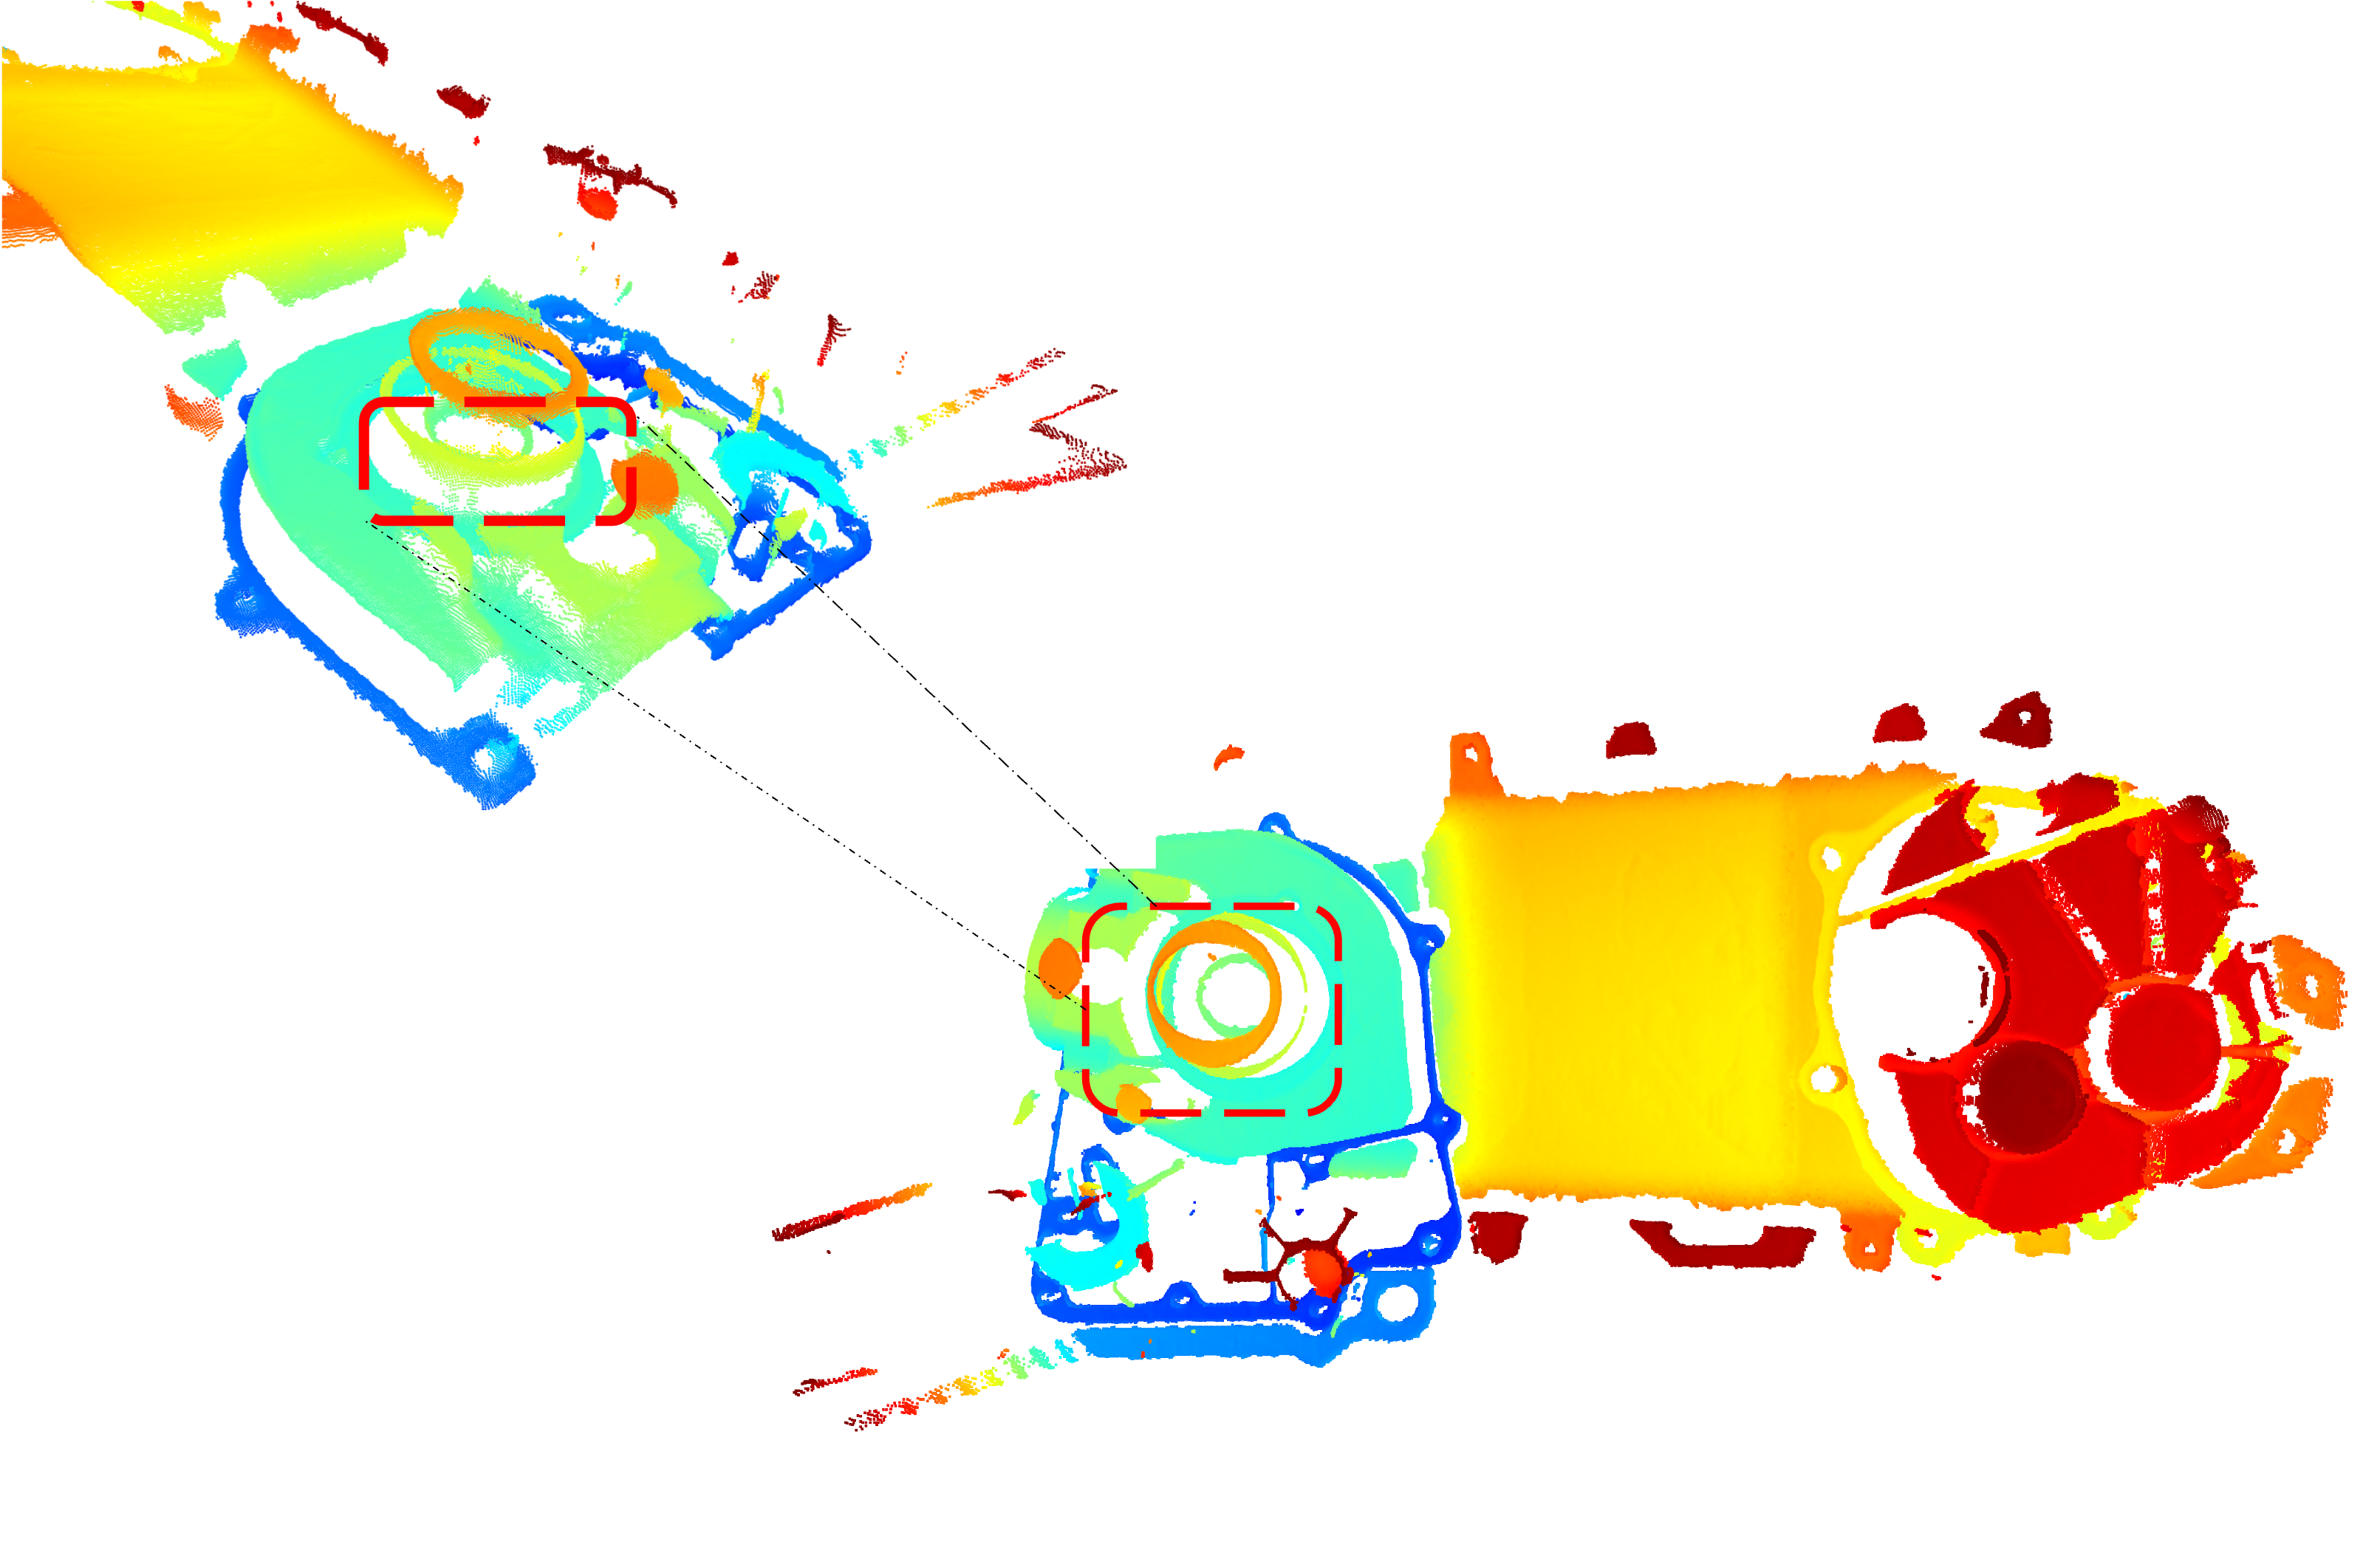
\includegraphics[width=0.75\textwidth]{figures/3/bad.png}
    \caption{结构缺陷样本示例}
    \label{fig:bad}
\end{figure}

此外,本文还引入了公开的3D缺陷检测数据集MVTec3D-AD\cite{bergmannMVTec3DADDataset2022},其包含有10种类型物体的训练和测试数据集。

\subsection{实验设计}
本文在Patchcore基础上引入的3D局部特征描述子RoPS是基于空间分布直方图来提取3D特征的,而3D局部特征描述子还有另一类是基于几何属性直方图的,其中以FPFH(Fast Point Feature Histograms)方法最为广泛应用,该方法将每个点的几何信息(例如,法线、曲率)和邻域关系转换为直方图表示。

因此本文以FPFH为基准设计对比实验,如表\ref{tab:3-experiment-desgin}所示。其中FPFH的直方图维数为,RoPS直方图的维数为135,两者均应用于点云降采样后的所有点。
\begin{table}[htbp]
    \centering
    \caption{金属工件数据集实验设计} \label{tab:3-experiment-desgin}
    \begin{tabular*}{0.6\textwidth}{@{\extracolsep{\fill}}ccc}
    \toprule
      &原理&直方图维数\\
      \midrule
        FPFH&几何属性&33\\
        RoPS	&空间分布&135\\
    \bottomrule
    \end{tabular*}
\end{table}

\subsection{实验结果和分析}
本文按照实验设计在正常样本组成的训练集上分别采用FPFH和RoPS提取3D特征并通过PillarCore聚合存储后,在自建的数据集和公开数据集上验证了算法的性能。实验采用的评价指标为在第二章中介绍的图像级的AUROC,其中在本文的金属件数据集上的实验结果如表\ref{tab:motor-experiment}所示。
\begin{table}[htbp]
    \centering
    \caption{金属工件数据集图像级AUROC} \label{tab:motor-experiment}
    \begin{tabular*}{0.4\textwidth}{@{\extracolsep{\fill}}cc}
    \toprule
      &金属工件\\
      \midrule
        FPFH&0.929\\
        RoPS	&0.96\\
    \bottomrule
    \end{tabular*}
\end{table}

从金属工件数据集实验结果中不难看出,本文引入RoPS作为3D局部特征提取提子的方法在本文的金属工件上的性能要优于FPFH方法。

\begin{table}[htbp]
    \centering
    \caption{MVTec3D-AD数据集图像级AUROC} \label{tab:mvtec3d-experiment}
    \begin{tabular*}{1\textwidth}{@{\extracolsep{\fill}}ccccccccccc}
    \toprule
      &百吉圈&密封套&萝卜&曲奇&暗榫&泡沫板&桃&土豆&绳索&轮胎\\
      \midrule
        FPFH&0.82&0.533&0.877&0.769&0.718&0.574&0.774&0.895&0.99&0.582\\
        RoPS&$\mathbf{0.868}$&$\mathbf{0.534}$&0.565&$\mathbf{0.989}$&$\mathbf{0.774}$&$\mathbf{0.692}$&0.77&0.819&0.834&0.577\\
    \bottomrule
    \end{tabular*}
\end{table}

在MVTec3D-AD数据集上的实验结果如表\ref{tab:mvtec3d-experiment}所示,其中黑色加粗表示在百吉圈、密封套、曲奇、暗榫以及泡沫板数据集上,本文引入RoPS的方法比FPFH的方法图像级AUROC指标高。从曲奇和萝卜两个数据集的图像级AUROC指标可以看出,基于空间分布的RoPS方法和基于几何分布的FPFH方法有各自擅长的点。两种方法在曲奇数据集上的ROC曲线如组图\ref{fig:cookie}所示,其中左图为FPFH方法,右图为RoPS方法。

\begin{figure}[htbp]
    \centering
    \begin{subfigure}
        \centering
        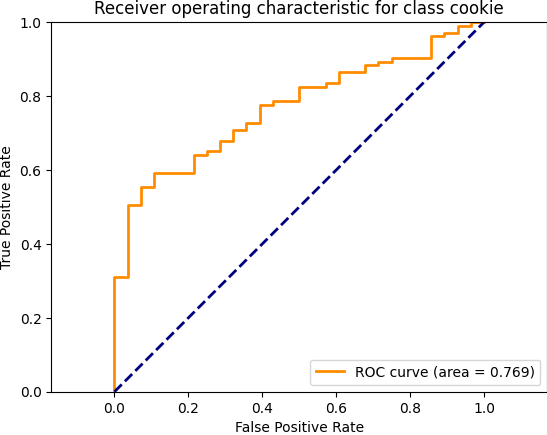
\includegraphics[width=.42\linewidth]{figures/3/cookie_FPFH.png}  
      \end{subfigure}
      \begin{subfigure}
        \centering
        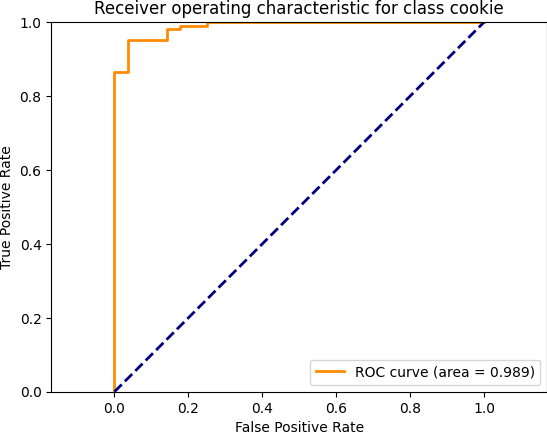
\includegraphics[width=.42\linewidth]{figures/3/cookie_RoPS.png} 
      \end{subfigure}
    \caption{曲奇数据集ROC曲线图}
    \label{fig:cookie}
  \end{figure}

\section{本章小结}
本章分别分别从整体算法框架、算法的输入处理方法(包括点云预处理、点云三角化及点云局部特征提取)和算法的核心处理方法三个角度介绍了本文提出的基于点云的面向非平整表面无监督缺陷检测算法PillarCore——通过引入RoPS特征提取方法将应用于二维图像缺陷检测的PatchCore方法迁移到三维数据,并在多个数据集和FPFH算法的对比实验中验证了本方法的有效性。

